% !TeX spellcheck = en_US
%MEGA MAN X2.TEX
\chapter{Game overview}
\textit{Mega Man X2} serves as a direct sequel to the inaugural \textit{Mega Man X} installment. Released in Japan on December 16 1994, and subsequently in North America and PAL regions in 1995, the sequel retains the gameplay mechanics and visual style of its precursor. Notably, Capcom incorporated the Cx4 enhancement chip into the cartridge, a technological advancement that facilitated the integration of 3D wireframe effects into the game. The development team received instructions to maximize the utilization of these effects throughout the game's design~\cite{wiki:MMX2}. However, an integral aspect of the game's localization involved a substantial script adaptation for the American version. This changes led to the omission of key details and connections within the plot, ultimately creating a more straightforward narrative, albeit at the cost of its comprehensive nature. Of particular note, this process changed all instances of X's name with \textit{Mega Man X}. To alleviate any potential confusion, this chapter will adhere to a translation directly from the Japanese game script, available in sources like \cite{wordpress:X2_japanese_script} and \cite{gamesfaq:X2_japanese_script}, in order to account for the entirety of plot-related events.

\begin{figure}[htp]
	\centering
	\begin{subfigure}[c]{0.5\linewidth}
		\centering
		
\includegraphics[height=4cm]{figures/X2/Mega_Man_X2_Box_Art.png}
	\end{subfigure}
	\begin{subfigure}[c]{0.3\linewidth}
		\centering
		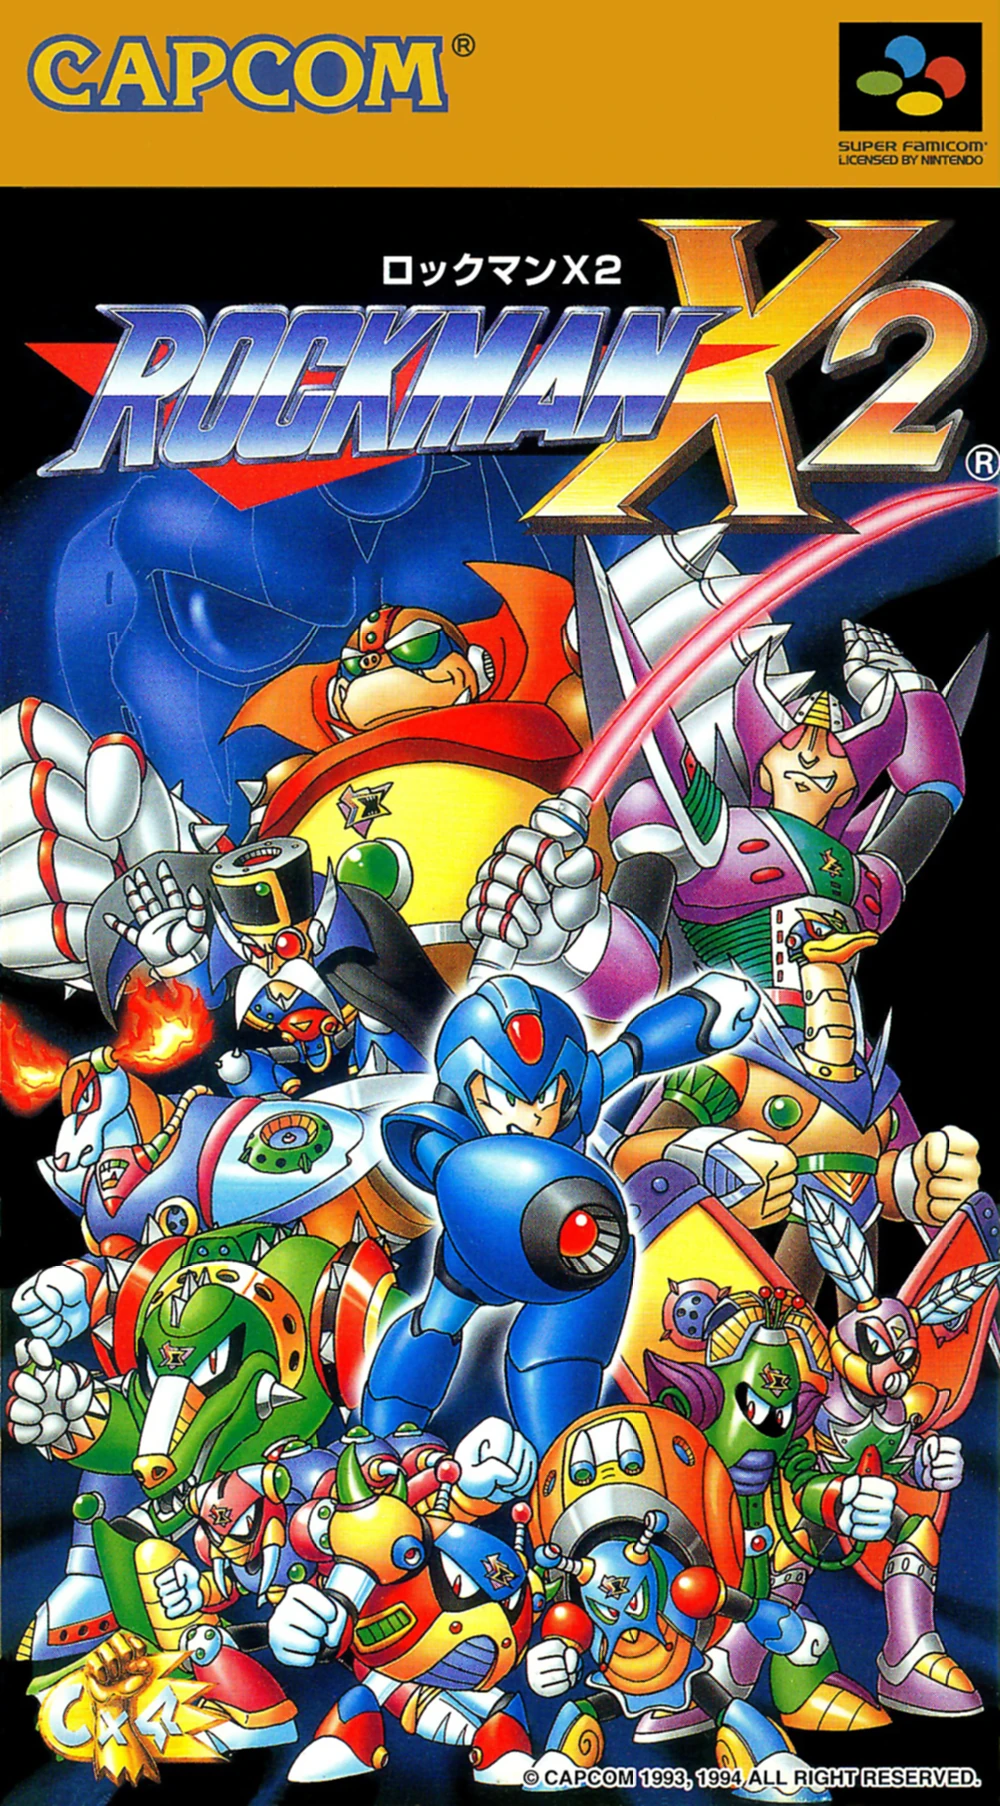
\includegraphics[height=4cm]{figures/X2/Rockman_X2_Box_Art.png}
	\end{subfigure}
	\caption{Cover art for the American and Japanese version of the game.}
\end{figure}


\section{Main plot}
Six months after X's victory over Sigma, the mavericks' threat continues to plague both humanity and reploids. Despite the ongoing efforts of the Maverick Hunters to restore peace, their numbers have been severely depleted, with only a quarter of their original force remaining due to the heavy losses incurred during the initial revolution~\cite{Xcoll1:Manual_X2}. Furthermore, the frequency of maverick attacks has escalated, and many Maverick Hunter bases have been destroyed. Surprisingly, the number of reploids joining Sigma's forces at the onset of his rebellion was relatively modest, therefore making the increasing threat more perplexing. By analyzing the defeated mavericks, scientists have discovered an anomalous chip bearing Sigma's emblem. This chip, embedded during the mavericks' creation, has been identified as the catalyst for their maverick transformation.
\begin{figure}[htp]
	\centering
	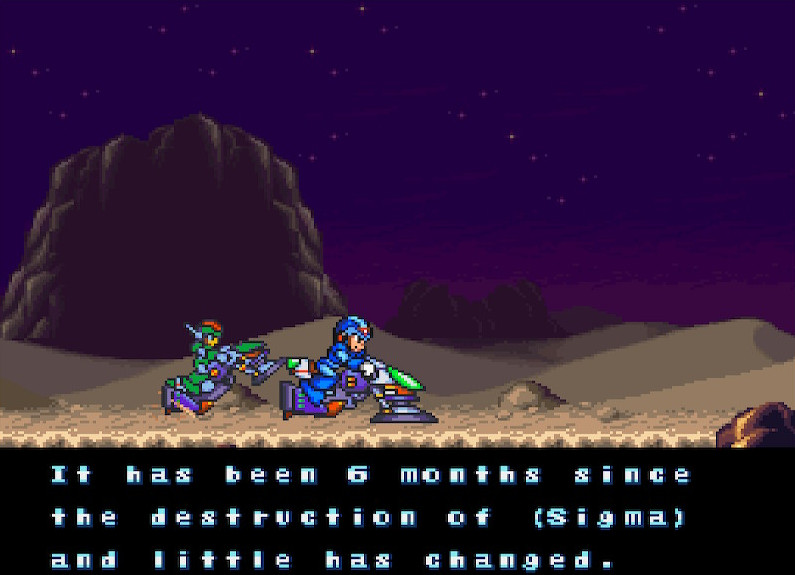
\includegraphics[height=3cm]{figures/X2/story_1.jpg}
	\caption {X attacking the maverick factory}
\end{figure}

 The Maverick Hunters manage to locate the factory responsible for manufacturing these corrupted reploids. During an operation against this facility, the events of Mega Man X2 begins. Following an intense battle outside the factory, X successfully infiltrates the facility  and ultimately obliterates it. The scene then shifts to reveal three shadowy figures observing X's actions on a monitor. The three acknowledge the potential threat X poses to their ambitions, despite remaining firmly sure of their superiority. Therefore, they keep observing him as he battles their eight SA-class maverick subordinates, thus granting them additional time to finalize their plans. 
\begin{figure}[htp]
	\centering
	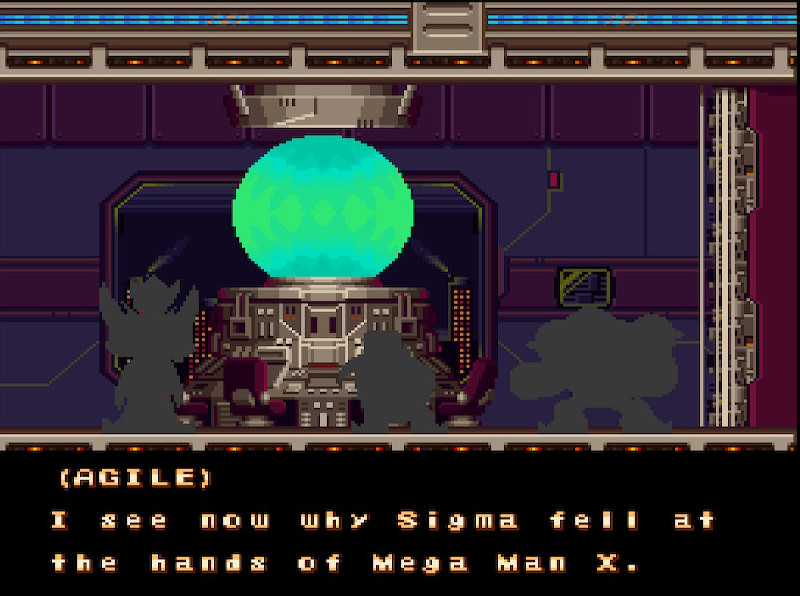
\includegraphics[height=3cm]{figures/X2/story_2.jpg}
	\caption {The X-Hunters realizing X's strength.}
\end{figure}
X, however, exceeds the expectations of these enigmatic figures by vanquishing the mavericks at a quicker pace than anticipated. Consequently, the three figures emerge from the shadows to directly confront X in an effort to hinder his progress and eliminate him. The three reveal their identities to the Maverick Hunter headquarters, introducing themselves as Agile, Serges, and Violen, collectively forming a group known as the ``X-Hunters'', and claim that their objective is to serve as a counterpart to the Maverick Hunters. Subsequently, they challenge X with a proposition: for each X-Hunter he successfully locates and defeats in a one-on-one confrontation, he will receive a piece of Zero's recovered and repaired body. X proceeds to accept the challenge, and resume his battle against the remaining mavericks.

The culmination of this journey leads X to the X-Hunter fortress, where the story branches into two possible outcomes based on X's success in defeating the X-Hunters and reclaiming Zero's parts. Should X successfully gather all of Zero's parts, Dr.~Cain undertakes the reparation process and identifies the X-Hunter fortress's location. If, however, X fails to retrieve at least one of Zero's parts, the X-Hunters infiltrate Dr. Cain's laboratory, confiscating all of Zero's components, including the control circuit necessary for his revival. Regardless of the outcome, the X-Hunter fortress's position is eventually traced to the North Pole.

Upon infiltrating the X-Hunter fortress, X encounters and confronts the X-Hunters once again. This time, however, their objective is not to merely slow him down but to eliminate him definitively: Violen adopts a more powerful form known as Neo Violen, Serges employs his Serges Tank, and Agile utilizes the Agile Flyer to stop X. Despite their enhanced efforts, all of the X-Hunters ultimately fall to X's determination. The X-Hunter plan however culminates with Sigma appearing before X in the fortress as it begins to self-destruct. Sigma challenges X to a final battle within the Central Computer, a location previously visited by X. The outcome of this battle depends on X's success in retrieving all of Zero's parts.
If Zero's parts remain incomplete, Sigma stands alongside a restored but unresponsive Zero, commanding him to attack X. After X defeats Zero in battle, he regains his consciousness, apologizes for his actions, and collaborates with X to open a path forward. In the event that X acquires all of Zero's parts, Sigma introduces a black replica of Zero and initiates an assault on X. The real Zero intervenes, easily disposing of the replica, and declares his allegiance to X. Zero subsequently enables X's progression by creating an opening for him.

\begin{figure}[htp]
	\centering
	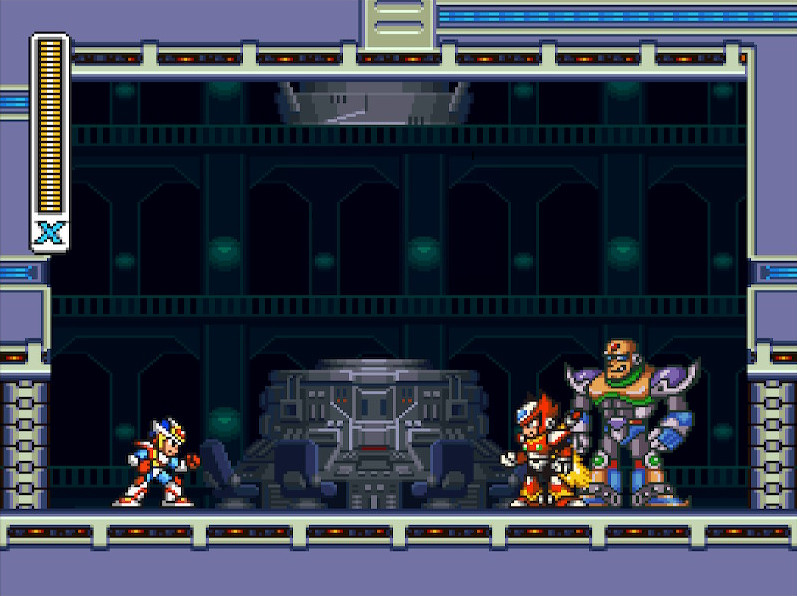
\includegraphics[height=3cm]{figures/X2/story_3_2.jpg}
	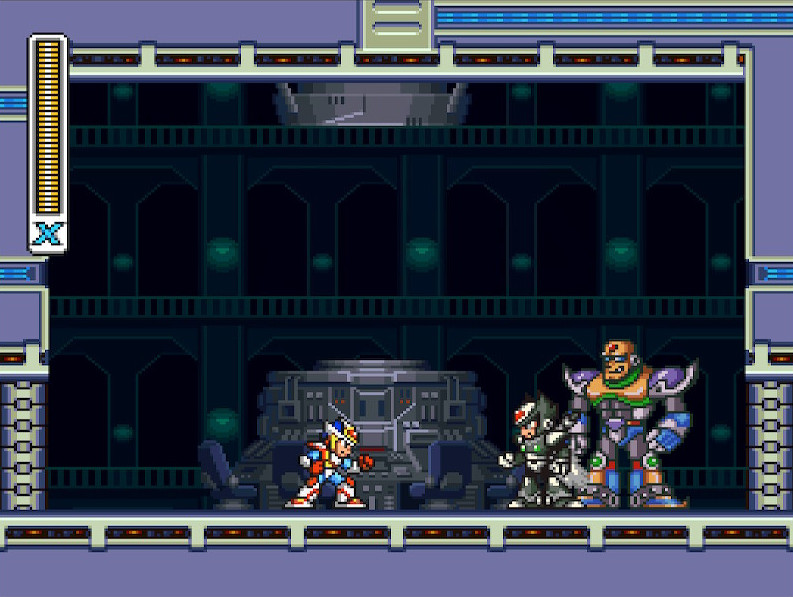
\includegraphics[height=3cm]{figures/X2/story_3.jpg}
	\caption{X against Sigma and Zero/Fake Zero.}
\end{figure}

Regardless of the circumstances, X eventually reaches the final confrontation with Sigma, who has acquired a new body. Similar to the previous game, X manages to defeat Sigma's physical form, only to uncover the truth: Sigma's real nature is that of a sentient virus capable of materializing in the real world. Following an intense battle, X emerges victorious, and Sigma disappears after issuing a final warning. This time, rather than blaming X for his plans' failure, Sigma warns that he will always find a way to match X's power, regardless of his level. Despite his ominous words, Sigma's lingering concern is the alliance between X and Zero. Sigma is surprised by the unexpected outcome, as he had firmly believed Zero would stand by his side, considering it almost a destiny.

Upon Sigma's defeat, X and Zero reunite near a seaside. In this poignant moment, X reflects on his purpose, the immense power within him, and the potential realization of the dream envisioned by Dr.~Light—a world where humans and reploids coexist in harmony.

\begin{figure}[htp]
	\centering
	
\includegraphics[height=3cm]{figures/X2/Ending.jpg}
	\caption{Game's ending scene}
\end{figure}
\section{Main Characters}

\subsection{X}

\begin{figure}[htp]
	\centering
	
\includegraphics[height=\portraitsize]{figures/X2/X.png}
	\caption{X as he appears in X2.}
\end{figure}

X, introduced in Chapter~\ref{char:X}, stands as Dr.~Light's final creation and serves as the reference model for the development of all reploids, despite his technology remaining enigmatic even to the scientific knowledge of his era. When Sigma initiated his rebellion against humanity, X emerged as the hero who confronted him. X's efforts stopped Sigma's plans, delivering an era of tranquility. Recognizing his valor, X was appointed as the leader of the 17th Elite Unit, a rank previously held by both Sigma and Zero, a dear companion to X, who ultimately sacrificed himself to safeguard his friend.

Although X's extraordinary abilities are well-established, his rank as an Hunter has remained unaltered. Nevertheless, some individuals have begun to perceive that X possesses latent potential capable of surpassing even the abilities of SA-ranked Hunters. Despite his incredible power, X remains a kindhearted person which refuse to believe violence is the only solution to the maverick problems, and the turmoil caused by his kind spirit and the need to fight to protect innocent is something very few people understand\cite{Xcoll1:Manual_X2}.

\subsection{Zero}

\begin{figure}[htp]
	\centering
	
\includegraphics[height=\portraitsize]{figures/X1/Zero_X1.png}
	
\includegraphics[height=\portraitsize]{figures/X2/Hunter_stages/Zero.png}
	\caption{Zero as he appeared in X1 and how appears from X2 onward.}
\end{figure}

As described in Chapter~\ref{char:Zero}, Zero is an SA-ranked Maverick Hunter affiliated with the 17th Elite Unit, and he stands as X's closest confidant and best friend. Their deep bond enables Zero to truly grasp X's sentiments and emotions. During the conflict with Sigma, Zero assumed leadership of the Maverick Hunters, guiding them in the battle against Sigma's uprising. Near the end of the conflict Zero was forced to detonate his energy core to protect his friend X, but at the cost of his life. Fortunately, Zero's control chip survived the explosion and was preserved within the Maverick Hunter headquarters.

Parallel to X's circumstances, repairing Zero's intricate body presents a challenge beyond Dr.~Cain's expertise. Nonetheless, the resourceful scientist Serges of the X-Hunters is able to not only reconstruct Zero's body but also enhance it, effectively resurrecting him as a Maverick~\cite{wayback:X2_resources} (subject to the specific ending achieved by the player). The responsibility for Zero's restoration and upgrades may fall to either Serges or Dr.~Cain, employing parts rebuilt by Serges. By the conclusion of the game, Zero makes his triumphant return. Depending on the player's choices, he either confronts X or destroys a duplicate of himself. Zero subsequently grants X a passage to confront Sigma. In the game's conclusion, Zero is depicted gazing out at the sea alongside his friend X, encapsulating their enduring companionship.

\subsection{Dr.~Cain}
\begin{figure}[htp]
	\centering
	
\includegraphics[height=\portraitsize]{figures/Characters/Char_Cain_X2.png}
	\caption{Dr~Cain.}
\end{figure}
Dr.~Cain, as detailed in Chapter~\ref{char:Cain}, stands as the greatest robotics expert in the 22nd century\cite{Xcoll1:Manual_X2}. By using the schematics developed by Dr. Light and with the assistance of X, Dr.~Cain alone was responsible for the transformation of robots in his era. He lead the world in the era of reploids, a new generation of robots  with the capacity for independent thought, action, and emotion. Regrettably, this advancement also gave rise to the emergence of mavericks, including the noteworthy Sigma, who incidentally was one of Dr.~Cain's most notable creations.

In the present, Dr.~Cain assumes the roles of both the founder of the Maverick Hunters organization and a pivotal figure within its vertexes. Throughout the events of the X2 games, Dr.~Cain serves as a guide, remotely coordinating X's operations and ultimately identifying the location of the X-Hunter base to facilitate the final assault. His contributions extend to supporting the Maverick Hunters' actions, exemplified by his efforts to restore Zero's physical form. However, these restoration efforts requires that X successfully procures  first all of the previously-repaired components from the X-Hunters.

\subsection{X-Hunters}
\begin{figure}[htp]
	\centering
	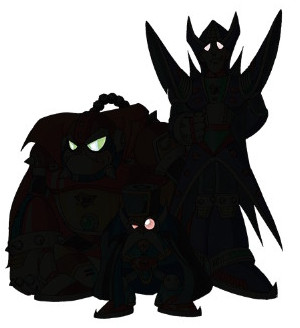
\includegraphics[height=\portraitsize]{figures/X2/Enemies/X_Hunters.jpg}
	\caption{The X-Hunters.}
\end{figure}

After the defeat of Sigma at the hands of X, it was believed that the wave of maverick attacks would cease, given the absence of a central leader to orchestrate them. However, reality would prove different as, rather than relenting, the maverick army swiftly regrouped under a new banner: the X-Hunters. This faction, led by three formidable reploids named Agile, Serges (more details in chapter \ref{char:Serges}), and Violen, assumed command of Sigma's former forces. Reorganizing the maverick army, the X-Hunters embarked on a two-fold plan to carry forth Sigma's aspirations. First, they sought to reinforce their ranks by capturing a reploid factory and repurposing it to implant special chips into produced reploids, brainwashing them into becoming obedient maverick soldiers. Additionally, within this facility, massive CF-0 reploids were constructed to further amplify their military power.

However, the most pivotal facet of the X-Hunters' strategy was the resurrection of Zero and Sigma. This scheme necessitated a considerable amount of time, as only Serges possessed the knowledge required to fabricate a new body for Sigma and restore the components of Zero they had salvaged. The absence of Zero's control circuit, the sole component preserved by the Maverick Hunters, further delayed their progress. To secure the window needed for their plan's completion, the X-Hunters deployed eight SA-ranked mavericks to strategic targets, with the intent of disrupt the Maverick Hunters' operations even more, after the loss of the maverick factory. However, their assessment of X's strength proved to be gravely underestimated, as X rapidly dispatched the deployed mavericks at a faster rate than anticipated by the X-Hunters'. Consequently, they found themselves in need to personally intervene and use their collection of Zero's restored components as incentives to engage X in battle, risking to forfeit a key element of their plans.

Depending on the player's progression, the X-Hunters could be either entirely defeated, compelling them to retreat to their fortress and change their scheme by constructing a fake replica of Zero, or they could survive their encounters with X and infiltrate the Maverick Hunters' headquarters, to steal all of Zero's components. The latter course would culminate in the complete resurrection of Zero as a maverick, although leaving behind a trail pointing to their hideout. Regardless of the outcome, X eventually locates the X-Hunters' stronghold and initiates his assault. To halt his advance, the trio opt to challenge X individually, using all available resources to attain superiority. However, each X-Hunter ultimately falls in battle.


\section{Game Mechanics}
As a direct sequel to \emph{Mega Man X}, Mega Man X2 maintains most of the gameplay mechanics present in the first title while introducing several new features and enhancements:
\begin{itemize}
	\item \textbf{Dashing}: X starts the game with the ability to dash, providing increased mobility. Additionally, this ability can be upgraded further to include air-dashing, allowing for greater maneuverability in mid-air.
	\item \textbf{Stage Interactions}: Unlike the first game, Mega Man X2 removes the concept of stage interactions. Completing a particular level no longer grants specific advantages in another stage
	\item\textbf{ X-Hunter Challenges}: After two bosses have been defeated, the three X-Hunters will start appearing in various remaining levels. Their movements can be tracked on the map screen whenever the player returns to it. To challenge an X-Hunter, the player needs to find a secret room within a stage, normally inaccessible. Defeating each X-Hunter grants X a part of Zero to resurrect his friend. If the player deliberately avoids the X-Hunter fights, the X-Hunters will flee permanently, resulting in the loss of the corresponding Zero part. 
	\item \textbf{Ride Chaser}: In a specific stage, X gains access to the Ride Chaser, a high-speed motorcycle. Unlike the Ride Armor, the Ride Chaser moves autonomously in the direction X is facing. It can jump and dash forward but cannot be stopped and if it collides with a wall, it will explode. Unlike the Ride Armor, the Ride Chaser doesn't provide protection to X, so he takes full damage when hit by enemies.
	\item \textbf{New Ride Armor}: This game features an upgraded Ride Armor from the previous game. This new version is controlled just as the precedent, but can also perform a charged dash attack, by keeping the fire button pressed, and hover for a short amount of time by pressing the jump button.
	\item \textbf{Desperation moves} for bosses: Starting from this game, certain bosses will change their attack pattern when below a certain HP threshold. This changes may include a phase change with increased damage or a desperation move, a more powerful attack usually during which the boss becomes invincible.
\end{itemize}

\section{Weapons}\label{X2:sub_weapon}
Here are now listed all sub-weapons available inside \textit{Mega Man X2}~\cite{wiki:X_weapons}

\subsection{\includegraphics[width=12px, height=10px]{figures/X2/weapons/C_Hunter.png} Crystal Hunter}\label{Crystal_Hunter}

Crystal Hunter fires a liquid glob that crystallizes upon contact with smaller enemies. Once crystallized, these enemies become immobilized and, if they were airborne, they fall to the ground. X has the option to utilize the created crystal as a platform for standing, or to dash through it, instantly shattering both the crystal and the encased enemy. Enemies vanquished in this manner will consistently drop a health capsule. Upon charging, this weapon creates a brief screen distortion and temporal deceleration, causing all on-screen entities (including X) to move at a reduced pace. Acquisition of this weapon is accomplished by defeating Crystal Snail~[\ref{boss:Crystal_snail}].

\begin{figure}[htp]
	\centering
		\includegraphics[height=3cm]{figures/X2/weapons/C_Hunter_1.png}	
		\includegraphics[height=3cm]{figures/X2/weapons/C_Hunter_2.png}	
	\caption{Crystal Hunter sub-weapon and trapped enemy.}
\end{figure}

\subsection{
\includegraphics[width=12px, height=10px]{figures/X2/weapons/B_splash.png} Bubble Splash}\label{Bubble_splash}
Bubble Splash is the weapon acquired by defeating Bubble Crab~[\ref{boss:Bubble_crab}]. When employed, it emits a stream of bubbles that slowly curve upward as they travel, bursting upon contact with adversaries. The quantity of bubbles discharged corresponds to how much the fire button is pressed: a light touch results in the creation of a few bubbles, whereas heavier pressure deploys up to a maximum of seven bubbles~\cite{wiki:Bubble_splash}. Sustaining pressure on the fire button leads to a continuous stream of fire, with new bubbles forming immediately after the preceding ones pop. Upon charging, this weapon generates multiple bubbles surrounding X, damaging foes they come into contact with. However, these orbital bubbles progressively draw upon X's energy, ultimately vanishing upon energy depletion. Additionally, as the charging process necessitates the continuous engagement of the fire button, X will concurrently release bubbles, thereby consuming energy in the process. Notably, in underwater environments, Bubble Splash manifests slight alterations: released bubbles exhibit a more rapid upward curve, and when charged, the weapon notably increase X's jumps height.

\begin{figure}[htp]
	\centering
		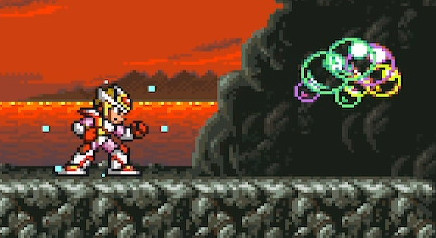
\includegraphics[height=3cm]{figures/X2/weapons/B_splash_1.jpg}	
		
\includegraphics[height=3cm]{figures/X2/weapons/B_splash_2.jpg}	
	\caption{Bubble splash normal fire and charged version.}
\end{figure}

\subsection{
\includegraphics[width=12px, height=10px]{figures/X2/weapons/S_shot.png} Silk Shot}\label{Silk_shot}
Upon triumphing over Morph Moth~[\ref{boss:Morph_moth}], X gains access to the Silk Shot. When employed, X propels a chunk of debris forward. When charged, X collects a substantial mass of debris towards him that remains affixed to the X Buster, serving as a shield as long as the fire button is held down. Upon releasing the button, the amassed debris is unleashed and detonates.

\begin{figure}[htp]
	\begin{subfigure}{\linewidth}
		\centering
		
\includegraphics[height=3cm]{figures/X2/weapons/S_shot_1.png}	
		
\includegraphics[height=3cm]{figures/X2/weapons/S_shot_2.png}	
		\caption{Crystals}	
	\end{subfigure}
	\begin{subfigure}{\linewidth}
		\centering
		
\includegraphics[height=3cm]{figures/X2/weapons/S_shot_3.png}	
		
\includegraphics[height=3cm]{figures/X2/weapons/S_shot_4.png}	
		\caption{Leafs}
	\end{subfigure}
\end{figure}
\begin{figure}
	\ContinuedFloat
	\centering
	\begin{subfigure}{\linewidth}
		\centering
		
\includegraphics[height=3cm]{figures/X2/weapons/S_shot_5.png}	
		
\includegraphics[height=3cm]{figures/X2/weapons/S_shot_6.png}	
		\caption{Rocks}	
	\end{subfigure}
	\begin{subfigure}{\linewidth}
		\centering
		
\includegraphics[height=3cm]{figures/X2/weapons/S_shot_7.png}	
		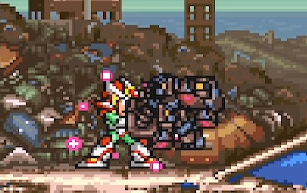
\includegraphics[height=3cm]{figures/X2/weapons/S_shot_8.png}	
		\caption{Scraps}
	\end{subfigure}
	\caption{Silk Shot attack types in normal and charged versions.}
\end{figure}
This weapon stands out as one of the most gimmicky in the entire series due to its dual attributes. Its main feature is its adaptability in terms of damage output and projectile characteristics varying on the stage in which it's utilized (the charged version remains largely unaltered, save for the material drawn), following the ensuing schema~\cite{wiki:Silk_shot}:
\begin{itemize}
\item In the \textbf{Energen crystal mine} stage, the weapon propels a crystal shard in the direction X faces, which bounce forward. Upon striking a wall, the crystal explodes in an X-shaped pattern.
\item In the \textbf{Weather Control stage}, the weapon launches an upward-floating collection of leaves. This version represents the weakest iteration of the Silk Shot.
\item In the \textbf{Volcanic Zone} and \textbf{Deep Sea base}, the weapon releases a rocky projectile that bounces once before detonating upon impact.
\item In all other stages, the weapon ejects a metallic fragment that immediately detonates upon touching any surface.
\end{itemize}

The second characteristic of this weapon lies in its capacity to attract health and energy capsules when its charged shot is employed within designated rooms in specific stages (refer to section~\ref{sec:refill}).


\subsection{
\includegraphics[width=12px, height=10px]{figures/X2/weapons/S_wheel.png} Spin Wheel}\label{Spinning_wheel}
When employing the Spin Wheel, X launches a buzz saw blade that descends to the ground before traversing along the floor. This blade consistently inflicts damage upon enemies it makes contact with, persisting until its dissipation or until the enemy is vanquished. In the latter scenario, the blade restarts its forward movement until it fades away. Additionally, the saw possesses the capability to obliterate specific blocks and terrain, thereby creating new pathways. However, only one blade can exist on-screen at any given time. Upon charging, X releases a blade that, instead of advancing forward, fragments into eight energy bolts that radiate in all directions. These bolts have the ability to penetrate obstacles and enemies, dealing damage while retaining the destructive attributes of the uncharged variant. The acquisition of this weapon requires first the defeat of Wheel Gator~[\ref{boss:Wheel_gator}].

\begin{figure}[htp]
	\centering
	\begin{subfigure}{0.4\linewidth}
		\centering
		
\includegraphics[height=3cm]{figures/X2/weapons/S_wheel_1.png}	
	\end{subfigure}
	\begin{subfigure}{0.3\linewidth}
		\centering
		
\includegraphics[height=3cm]{figures/X2/weapons/S_wheel_2.png}	
	\end{subfigure}
	\caption{Spin Wheel normal and charged version.}
\end{figure}

\subsection{
\includegraphics[width=12px, height=10px]{figures/X2/weapons/S_slicer.png} Sonic Slicer}\label{Sonic_slicer}
Following the victory over Overdrive Ostrich~[\ref{boss:Overdrive_ostrich}], X attains the ability to wield the Sonic Slicer. This armament projects a rotating blade that traverses horizontally at remarkable velocity, bouncing off walls at escalating angles of reflection with each collision. The blade persists until striking an enemy or exiting the screen.

Upon charging, this weapon releases a cluster of five closely spaced blades that ascend vertically. Subsequently, they separate and fall, getting bigger as they descend.
\begin{figure}[htp]
		\centering
		
\includegraphics[height=2.5cm]{figures/X2/weapons/S_slicer_1.png}	
		
\includegraphics[height=2.5cm]{figures/X2/weapons/S_slicer_2.png}	
		\vspace{2pt}\\
		
\includegraphics[height=2.5cm]{figures/X2/weapons/S_slicer_3.png}	
	\caption{Sonic Slicer normal and charged version.}
\end{figure}

\subsection{
\includegraphics[width=12px, height=10px]{figures/X2/weapons/S_chain.png} Strike Chain}\label{Strike_chain}
\begin{figure}[htp]
	\centering
	
\includegraphics[height=2.5cm]{figures/X2/weapons/S_chain_1.png}	
	
\includegraphics[height=2.5cm]{figures/X2/weapons/S_chain_2.png}	
	\caption{Strike Chain normal and charged version.}
\end{figure}
Upon utilizing the Strike Chain, X deploys a chain with a hook at its terminal end, capable of inflicting damage upon enemies it comes into contact with. The chain's extension is proportional to how much the fire button is held down: a brief press yields a slight extension, while a prolonged press stretches the chain to its maximum reach. Beyond its offensive capacity, the chain possesses the ability to collect items from a distance, including drops from enemies. Moreover, if the chain strikes a wall, it pulls X towards it. Upon charging, X discharges a swifter and longer chain that also delivers increased damage. Notably, enemies defeated by this method always drop an energy pickup for X.

\begin{figure}[htp]
	\centering
	
\includegraphics[height=2.5cm]{figures/X2/weapons/S_chain_grub.jpg}	
	\caption{Strike Chain grab ability.}
\end{figure}
The acquisition of this weapon requires the defeat of Wire Sponge~[\ref{boss:Wire_sponge}].

\subsection{
\includegraphics[width=12px, height=10px]{figures/X2/weapons/M_mine.png} Magnet Mine}\label{Magnet_mine}

Following the defeat of Magna Centipede~[\ref{boss:Magna_centipede}], X gains the ability to wield the Magnet Mine. This armament projects an individual mine that maintains a constant speed in the direction of its launch. Upon making contact with an enemy, the mine detonates; however, if it strikes a surface, it remains stationary momentarily before detonation. Once affixed to a surface, X can promptly launch another mine, allowing it to stack atop the preceding one, forming a linked sequence. There exists virtually no strict limit on the number of mines X can deploy, but typically only four can be launched prior to the initial one exploding.
\begin{figure}[htp]
	\centering
	\begin{subfigure}{0.4\linewidth}
		\centering
		
\includegraphics[height=3cm]{figures/X2/weapons/M_mine_1.png}	
		\caption{Normal fire}
	\end{subfigure}
	\begin{subfigure}{0.4\linewidth}
		\centering
		
\includegraphics[height=3cm]{figures/X2/weapons/M_mine_2.png}	
		\caption{Three mines stacked.}
	\end{subfigure}
	\end{figure}
	\begin{figure}[htp]
		\ContinuedFloat
		\centering
	\begin{subfigure}{0.4\linewidth}
		\centering
		
\includegraphics[height=3cm]{figures/X2/weapons/M_mine_3.png}	
		\caption{Charged version}
	\end{subfigure}
	\begin{subfigure}{0.4\linewidth}
		\centering
		
\includegraphics[height=3cm]{figures/X2/weapons/M_mine_4.png}	
		\caption{Absorbing incoming projectiles}
	\end{subfigure}
\end{figure}
\begin{figure}[htp]
	\ContinuedFloat
	\centering
	\begin{subfigure}{0.4\linewidth}
		\centering
		
\includegraphics[height=3cm]{figures/X2/weapons/M_mine_5.png}	
		\caption{Charged version second stage}
	\end{subfigure}
	\begin{subfigure}{0.4\linewidth}
		\centering
		
\includegraphics[height=3cm]{figures/X2/weapons/M_mine_6.png}	
		\caption{Charged version max size}
	\end{subfigure}
	\caption{Magnet Mine sub-weapon.}
\end{figure}
 Notably, each mine's vertical trajectory can be manipulated by inputting up or down; once a trajectory is chosen, the mine continues along that path. To revert it to a straight path, continuous upwards and downwards input is necessary. Upon charging, the weapon discharges a small black hole that advances slowly. This black hole can be controlled in a manner akin to the basic version (refer to \path{videos/X2/Charged_mine_control.mp4}). The black hole persists in its forward movement, traversing obstacles and damaging enemies and absorbing incoming projectiles, gradually expanding up to two stages in size. However, it also becomes more challenging to control as it grows.


\subsection{
\includegraphics[width=12px, height=10px]{figures/X2/weapons/S_burner.png} Speed Burner}\label{Speed_burner}
Upon acquiring the Speed Burner, X's X-Buster launches a pair of intertwined fireballs that race forward at a rapid pace, maintaining a straight trajectory until colliding with either an enemy or a surface, where they vanish. Furthermore, if the Speed Burner is activated while X is grounded, it leaves behind a diminutive trail of fire that inflicts damage upon enemies as well. Upon charging, this weapon surround X in flames, propelling him into a swift forward dash that damages adversaries. During this state, X is immune to contact damage from enemies, though he remains vulnerable to environmental hazards like spikes. This maneuver can be executed in mid-air, granting X the ability to perform an airborne dash.

\begin{figure}[htp]
	\centering
		\centering
		
\includegraphics[height=2cm]{figures/X2/weapons/S_burner_1.png}	
		
\includegraphics[height=2cm]{figures/X2/weapons/S_burner_2.png}\vspace{2pt}\\	
		
\includegraphics[height=2cm]{figures/X2/weapons/S_burner_3.png}	
		
\includegraphics[height=2cm]{figures/X2/weapons/S_burner_4.png}	
	\caption{Speed Burner sub-weapon attacks outside and inside water.}
\end{figure}

As observed in the prior game, the behavior of this fire-based weapon alters underwater. In this instance, when executing the regular attack, the two fireballs do not ignite in the aquatic environment. Instead, two minor orbs are emitted, causing minimal damage, and leaving behind a trail of smoke. Conversely, when the charged version is deployed, X performs a straightforward dash, again producing a trail of smoke. While in this state underwater, X lacks invincibility, rendering him susceptible to damage upon contact with an enemy. This weapon in integrated into X's arsenal only after vanishing Flame Stag~[\ref{boss:Flame_stag}] first.

\section{Second Armor}\label{X2:Armor}
Returning from the previous game, Dr.~Light's capsules once again hold new armor components. These components are distributed throughout four of the eight stages, albeit more hidden, often necessitating specific sub-weapons (or even other parts) to access them. Unlike the previous game, this installment doesn't feature any obligatory capsules, rendering the armor entirely optional.
\begin{figure}[htp]
	\centering
	\includegraphics[height=\portraitsize]{figures/X2/X2armor.png}
	\caption{The Second Armor.}
\end{figure}
According to \cite{tw:second_armor}\footnote{Translation: \url{https://twitter.com/kobun20/status/1305162448878612480}}, the second armor represents an enhanced iteration of the first. Following the event of the first game, X returned the armor to Dr. Light's capsule, which subsequently analyzed the armor's field data and proceeded to upgrade it.

The second armor, much like its predecessor, is composed of four core parts, with an additional fifth secret part, similar to the first game's Hadoken.
\begin{itemize}
\item \emph{Foot Parts}: These parts, once equipped, allow X to execute mid-air dashes. However, air dashes cannot be performed if X has already dashed on the ground or during a dash-jump. The distance covered during an air dash can be extended by combining the Foot Parts with a charged Speed Burner. The capsule containing this power-up is concealed within the Desert Base, obscured behind a breakable wall accessible only via the Spin Wheel sub-weapon.

\item \emph{Body Parts}: Similar to the previous game, this upgrade boosts X's defense by halving all incoming damage. Additionally, every instance of damage sustained by X contributes to a special gauge. Once this gauge is fully charged, X can execute the \textit{Giga Crush} attack, which inflicts significant damage upon all on-screen enemies. However, the gauge does not refill between stages, meaning that energy can only be accumulated by absorbing hits. The capsule for the Body Parts is concealed in the Robot Junkyard stage, beneath a floor at the initial stage section. This floor is destructible solely through the use of the Spin Wheel sub-weapon.
\begin{figure}[htp]
	\centering
	\includegraphics[height=3cm]{figures/X2/weapons/G_crush_1.png}
	\caption{Giga Crush attack.}
\end{figure}

\item \emph{Arm Parts}: This enhancement enables X to wield two X-Busters when employing a charged shot. While charging, X can surpass the initial charge level, stockpiling energy in the secondary Buster, up to two levels. Upon releasing the fire button, X discharges a first charged shot based on the reached charge level, and will remain pulsating. If the fire button is pressed again during this pulsating phase, X unleashes a fully charged second shot. Notably, if both charged shots are discharged in rapid succession, they can combo against enemies, including bosses, bypassing their invincibility frames and delivering substantial damage. This upgrade is located within the Wheel Gator stage, hidden within a chamber accessible through wall jumping from an opening in the roof. The room can be reached through precise wall-jumping, utilizing the Giga Crush to extend X's airborne duration, utilizing the Strike Chain to draw X towards the wall (\path{videos/X2/Buster_capsule_chain.mp4}), or simply by employing the air dash to access the opening.
	\begin{figure}[htp]
	\centering
	\includegraphics[height=2cm]{figures/X2/weapons/Double_shot.png}
	\caption{Double charged shot.}
\end{figure}

\item \emph{Head Parts}: These parts equip X with the item tracer, a radar that X can activate and which indicates the direction of the nearest hidden element within the stage. Identified secrets include secret passages and items such as heart tanks, sub-tanks, Light's capsules, and refill rooms. Despite featuring an ammunition gauge, this upgrade consumes no energy. The capsule housing the Head Parts is hidden in Crystal Snail's stage, found at the conclusion of a secret path accessible while sliding down a pit after defeating the stage's sub-boss.
\begin{figure}[htp]
	\centering
	\includegraphics[height=3cm]{figures/X2/weapons/Tracer.png}
	\caption{Item Tracer.}
\end{figure}

\item Shoryuken\label{shoryuken}: Analogous to X1's Hadoken, this secret enhancement is unlocked upon collecting all other power-up items (excluding Zero's parts). Once obtained, X gains the ability to execute the fire uppercut from the \textit{Street Fighter} series by inputting the command $\rightarrow$, $ \downarrow$, $\searrow$ (with X facing left) + fire button. However, this can only be executed when X is on solid ground and at full health. Differing from the previous technique, the damage inflicted by this attack is determined by the duration of contact with the enemy, potentially leading to instances where a mistimed Shoryuken fails to instantly defeat bosses.
	\begin{figure}[htp]
	\centering
	\includegraphics[height=3cm]{figures/X2/weapons/Shoryuken.png}
	\caption{Shoryuken.}
\end{figure} Precisely, the Shoryuken inflicts 16 damage to enemies without invincibility frames and 8 damage otherwise, delivered every two frames. Consequently, to vanquish a full-health boss (32 hit points), a minimum of 5 frames of contact is required (16 damage on the first frame, no damage on the second, 8 damage on the third, no damage on the fourth, and 8 damage on the fifth). The only bosses which escapes this rule are Flame Stage, who will take only 8 points of damage from the initial hit, thus requiring two more contact frame for being kill, and Morph Moth, as the boss fight will force his transformation regardless of the attack and ignoring any additional damage until the second phase has begun. This upgrade is located within the third X-Hunter stages, found at the conclusion of a concealed passage filled with spikes that necessitates an accurate air dash. Moreover, to acquire this capsule, X must reach it at full health, but there are no restrictions regarding Sub Tank status.
\end{itemize}

\chapter{Stages}	

\section{Opening Stage}
As the game's first stage, this level serves as a tutorial to (re-)introduce the player with fundamental game mechanics. The stage begins with a brief scene depicting X and other Hunters riding their vehicles toward a factory, only to encounter a fierce opposition. Following an attack, X dismounts his bike, which collides with an enemy and crashes. Taking control of X at this point, the player can start moving, albeit with caution, as the enemy hit by the bike is still active and will promptly fire at X. Beyond this initial obstacle, the player enters the factory where additional enemies await.

Traversing the factory leads X to a production line, which employs conveyor belts to transport constructed mavericks from one assembly bay to another (for a total of three bays). If X gets caught within one of these bays, he will sustain damage. However, passing over a bay will simply enhance the assembled maverick and, in the case of the third and final bay, the enhanced maverick will activate and engage X. Near the end, a brief tutorial on wall-jumping occurs: a \hyperlink{enem:Slidame}{Slidame}, upon detecting X, will swiftly ascends to the top of the room and initiates to close of the walls, aiming to crush X. Although not excessively fast, the player must climb the wall quickly enough to evade being crushed. If the player falls back to the room's base and the walls close, just briefly going back to reset the room  will provide another opportunity to climb.

Upon reaching the room's summit, a narrow corridor follows, concluding with a deep pit that X must jump into. At the pit's end awaits a boss door.

Beside enemies already cited, this level also house following enemies~\cite{wiki:X2_opening}:
\begin{itemize}
	\item \hyperlink{enem:Bar_Waying}{Bar Waying}
	\item \hyperlink{enem:Cannon_Driver}{Cannon Driver}
	\item \hyperlink{enem:Mecha-Arm}{Mecha-Arm}
	\item \hyperlink{enem:Scrambler}{Scrambler}
	\item \hyperlink{enem:Scriver}{Scriver}
	\item \hyperlink{enem:Slidame}{Slidame}
\end{itemize}

\subsection{Giant Mechaniloid CF-0}
\begin{figure}[htp]
	\centering
	\includegraphics[height=\portraitsize]{figures/X2/Enemies/CF0.png}
	\includegraphics[height=\portraitsize]{figures/X2/Enemies/Gigantic_Mechaniloid_CF0.png}
	\caption{Giant Mechaniloid CF-0's artwork~\cite{book:MMX_Complete_art} and X Dive's artwork}
\end{figure}
In contrast to the previous game, this introductory stage culminates in a boss battle. The antagonist in question is the \emph{Giant Mechaniloid CF-0}, a robot engineered by the X-Hunters for the purposes of mass production and the conquest of global cities. However, due to its substantial weight, its mobility turned out to be severely hindered. The X-Hunters' ambitions to deploy CF-0s were halted by an offensive from Maverick Hunters, forcing them to activate the solitary completed mechaniloid in an attempt to stop the assault. Regrettably for them, their effort resulted in CF-0's demise at the hands of X.
\begin{figure}[htp]
	\centering
	\begin{subfigure}{0.4\linewidth}
		\centering
		\includegraphics[height=3cm]{figures/X2/cf_punch.jpg}
		\caption{CF-0 punching}
	\end{subfigure}
	\begin{subfigure}{0.4\linewidth}
		\centering
		\includegraphics[height=3cm]{figures/X2/cf_walk.jpg}
		\caption{CF-0 walking around}
	\end{subfigure}
	\caption{Giant Mechaniloid CF-0's attacks.}
\end{figure}
Despite its imposing size, the confrontation with CF-0 is relatively straightforward. The boss chamber is big enough and contains platforms at various heights, interconnected by ladders to facilitate X's ascent should he fall. This design allows X to easily avoid the two attacks that CF-0 can execute: a spiked \emph{Punch} targeting X's position and a jumping \emph{Kick} where CF-0 aims to land on X. Both these attacks can be evaded effortlessly by moving among the upper platforms, and even if they connect, they inflict minimal damage to X.

The optimal strategy is to remain on the upper layers of the room to attack the boss, as its sole vulnerable point is the head. Curiously, the head along with CF-0's arms and feet are the body parts capable of causing damage to X upon contact, since the remaining portions of CF-0's body act as part of the background. Notably, despite possessing a boss-level health bar, CF-0 sustains massive damage from X's charged shot, which can obliterate it in a mere four shots. Following the boss' defeat a small scene will play culminating in the classical world map, presenting the eight boss to fight against.

\begin{table}[htp]
	\centering
	\begin{tabular}[h]{l c}
		\toprule
		\multicolumn{1}{c}{Health}  & 32\\
		\midrule
		\multicolumn{1}{c}{Attack} & \multicolumn{1}{c}{Damage}\\
		Punch & 2 \\
		Kick & 2 \\
		\bottomrule
	\end{tabular}
	\caption{Giant Mechaniloid CF-0's attacks~\cite{wiki:CF-0,book:Compendium}}
\end{table}

 As tradition, players are free to choose the order in which challenge these enemies as they wish.
\begin{figure}[htp]
	\centering
	\includegraphics[width=0.5\linewidth]{figures/X2/map.png}
	\caption{Full map with Bosses and their locations}
\end{figure}


\section{Weather Control Center}

The first stage the game presents is the weather control stage. As the name suggests, the central theme of this stage revolves around weather conditions, which can transform and be manipulated as the stage unfolds. The catalyst for these weather shifts is introduced right at the beginning of the level: the \hyperlink{enem:Weather_crystal}{weather crystals}. Although categorized as enemies, these entities pose no threat to X upon contact. Instead, they alter the weather conditions within the sector of the level where X is situated, impacting his movement and affecting enemy attributes. While this may initially appear to be a hindrance, X can exploit these enemies to generate favorable weather conditions that facilitate stage exploration. The stage counts four weather crystals in total, each assigned a default weather pattern that can be transformed by striking the crystal with a specific weapon, as detailed in the following list~\cite{wiki:Weather_crystal}:

\begin{figure}[htp]
	\centering
	\begin{subfigure}{0.3\linewidth}
		\centering
		\includegraphics[width=\linewidth]{figures/X2/Wire_sponge/sponge_crystal_default.jpg}
		\caption{Intact crystal}
	\end{subfigure}
	\begin{subfigure}{0.3\linewidth}
		\centering
		\includegraphics[width=\linewidth]{figures/X2/Wire_sponge/sponge_crystal_cloud.jpg}		
		\caption{Cloudy}
	\end{subfigure}
	\begin{subfigure}{0.3\linewidth}
		\centering
		\includegraphics[width=\linewidth]{figures/X2/Wire_sponge/sponge_crystal_sun.jpg}
		\caption{Sunny}
	\end{subfigure}
	\begin{subfigure}{0.3\linewidth}	
		\centering
		\includegraphics[width=\linewidth]{figures/X2/Wire_sponge/sponge_crystal_rain.jpg}\\
		\caption{Rainy}
	\end{subfigure}
	\begin{subfigure}{0.3\linewidth}
		\centering
		\includegraphics[width=\linewidth]{figures/X2/Wire_sponge/sponge_crystal_fog.jpg}
		\caption{Foggy}	
	\end{subfigure}
	\begin{subfigure}{0.3\linewidth}
		\centering
		\includegraphics[width=\linewidth]{figures/X2/Wire_sponge/sponge_crystal_broken.jpg}
		\caption{Broken crystal}	
	\end{subfigure}
	\caption{Different states of weather condition and crystals.}
\end{figure}
\begin{itemize}
\item \textbf{Cloudy Weather}: Induced by employing the Strike Chain weapon on the crystal (causing it to turn yellow). During this state, all enemies are active and \hyperlink{enem:Sky_Farmer}{Sky farmers} will sow \hyperlink{enem:Sabottein}{sabotteins} that grow to half their maximum size.

\item \textbf{Warm/Sunny Weather}: Triggered by employing the Speed Burner on the crystal (causing it to turn orange). All enemies remain active, but \hyperlink{enem:Croak_hopper}{croak hoppers} overheat and explode, while planted \hyperlink{enem:Sabottein}{sabotteins} reach full growth.

\item \textbf{Rainy Weather}: Initiated by utilizing the Bubble Splash on the crystal (causing it to turn cyan). During this state, \hyperlink{enem:Croak_hopper}{croak hoppers} actively move across the stage instead of remaining stationary, \hyperlink{enem:Sky_Farmer}{Sky farmers} release \hyperlink{enem:Rightod}{rightods} to pursue X, and \hyperlink{enem:Sole_solar}{sole solars} are rendered inactive. Rainy weather also calls up wind to oppose X's movements, resulting in slower walking, running, and reduced jump distances.

\item \textbf{Foggy Weather}: Achieved by utilizing the Crystal Hunter on the crystal (causing it to turn purple/black). All enemies are deactivated in this state.
\end{itemize}

If a crystal is destroyed, the weather conditions within that segment of the stage will be randomized.

The first crystal is encountered early in the level, within a straightforward section featuring a few enemies. This area culminates in a second weather crystal, signaling the transition to the subsequent segment. Here, floating platforms oscillate vertically over a pit filled with spikes. X must navigate between these platforms, utilizing wall-jumping techniques since the platforms are taller than they are wide. The primary challenge in this area arises from the default rainy weather, which reduces X's jumping capability, making it more arduous for the player to move between platforms. The third section closely resembles the first, but with an elevated number of enemies and spiked pits. In this portion, the last two weather crystals can be located. Upon surmounting this segment, a climbing challenge awaits, incorporating platforms with enemies atop them, connected by ladders. This sequence concludes with a corridor leading to the boss door.

Following enemies occupy the stage~\cite{wiki:weather_control}
\begin{itemize}
	\item \hyperlink{enem:Aclanda}{Aclanda}
	\item \hyperlink{enem:Croak_hopper}{Croak Hopper}
	\item \hyperlink{enem:Rightod}{Rightod}
	\item \hyperlink{enem:Sabottein}{Sabottein}
	\item \hyperlink{enem:Scriver}{Scriver}
	\item \hyperlink{enem:Sky_Farmer}{Sky Farmer}
	\item \hyperlink{enem:Sole_solar}{Sole Solar}
	\item \hyperlink{enem:Weather_crystal}{Weather Crystal}
\end{itemize}


\subsection{Heart Tank}
The Heart Tank is hidden immediately at the beginning of the stage. By climbing the leftmost wall of the initial room, the player will find a small hidden entrance in the top corner with the Heart Tank inside it.

\begin{figure}[htp]
	\centering
		\includegraphics[height=3cm]{figures/X2/Wire_sponge/Sponge_heart.jpg}
		\caption{Heart Tank location.}
\end{figure}

\subsection{X-Hunter' room}
When reaching the elevator section, if player manage to make X sneak under the elevator a new path will open, leading to the X-Hunter room
	\begin{figure}[htp]
	\centering
	\includegraphics[height=3cm]{figures/X2/Wire_sponge/Sponge_Hunter_room.jpg}
	\caption{X-Hunter room location.}
\end{figure}

\subsection{Sub Tank}
In the rainy section, if instead of proceeding by platforming onto the logs X uses the first one to jump backwards onto the right wall (near where the second crystal is found) and climb it, he will reach a new path over the default one made of logs separated into two main platforms. At the end of the second one is where the Sub Tank resides.  
\begin{figure}[htp]
	\centering
	\includegraphics[height=3cm]{figures/X2/Wire_sponge/Sponge_tank.jpg}
	\caption{Sub Tank location.}
\end{figure}


\subsection{Wire Sponge}\label{boss:Wire_sponge}
Wire Sponge, known as the ``\textit{Little Forest Demon}''\cite{book:MMX_Complete_art}, was an SA-class Maverick with a sponge cucumber-based composition, manufactured within one of Sigma's factories. However, Wire Sponge's creation was the result of an unintended incident, as due to a design flaw, he was built with a personality disorder rendering him childlike, cheerful, and easily entertained. He also had a love for dancing and playing.
\begin{figure}[htp]
	\centering
	\includegraphics[height=\portraitsize]{figures/X2/Wire_sponge/Wire_Sponge.png}
	\caption{Wire Sponge's artwork~\cite{book:MMX_Complete_art}}
\end{figure}
 While this personality trait wasn't tailored for military purposes, Wire Sponge's strength and capacity for violence were unparalleled. The X-Hunters capitalized on these attributes, assigning him the task of conquering the weather control center, which he transformed into his own playground, manipulating the weather as he wished\cite{wiki:wire_sponge,wayback:X2_resources}.

In combat Wire Sponge primarily employs his Strinke Chain to execute various attacks against X. He can deflect incoming projectiles using his \emph{Chain Spin}, rendering attacks during this state ineffective. After spinning the chain, Wire Sponge usually throws it at X (\emph{Strike chain}) and, if the chain connects with a wall, he will be pulled towards it. Alternatively, Wire Sponge may hurl the chain onto the ceiling and ascend while launching seeds from his head toward X (\emph{Hanging}). Upon connecting with a wall or the floor (but not the ceiling, against which the seeds bounce), these seeds transform into spiked vines that harm X on contact. These spikes can be destroyed by any weapon, which is recommended, as after planting four vines Wire Sponge will descend~\cite{rta:x2}.\begin{figure}[htp]
	\centering	
	\begin{minipage}[b]{0.4\linewidth}		
		\begin{subfigure}{\linewidth}
			\centering
			\includegraphics[height=3cm]{figures/X2/Wire_sponge/Sponge_spin.png}
			\caption{Spinning the chain}
		\end{subfigure}
		\begin{subfigure}{\linewidth}
			\centering
			\includegraphics[height=2cm]{figures/X2/Wire_sponge/Sponge_pull.jpg}
			\caption{Being pulled to the wall}
		\end{subfigure}
	\end{minipage}
	\begin{minipage}[b]{0.4\linewidth}		
		\centering
		\includegraphics[height=5.3cm]{figures/X2/Wire_sponge/Sponge_hang.jpg}
		\caption{Launching seeds.}
	\end{minipage}
\end{figure} Therefore, since this move is the one which exposed Sponge the most, it is optimal to prolong its execution by destroying such vines as they appear.
\begin{figure}[htp]
	\ContinuedFloat
	\centering
	\begin{subfigure}{\linewidth}
		\centering
		\includegraphics[height=3cm]{figures/X2/Wire_sponge/Sponge_phase2.jpg}
		\includegraphics[height=3cm]{figures/X2/Wire_sponge/Sponge_DM.jpg}
		\caption{Charging and releasing his desperation move}
	\end{subfigure}
	\begin{subfigure}{0.35\linewidth}
		\centering
		\includegraphics[height=3cm]{figures/X2/Wire_sponge/Sponge_charged.jpg}
		\caption{Powered up by electricity}
	\end{subfigure}
	\begin{subfigure}{0.35\linewidth}
		\centering
		\includegraphics[height=3cm]{figures/X2/Wire_sponge/Sponge_cut.jpg}
		\caption{Cut in half.}
	\end{subfigure}
	\caption{Wire Sponge's attacks.}
\end{figure}
When Wire Sponge's health drops below 10 points, he will initiate his desperation move, \emph{Lightning Strike}. During this phase, his flower becomes a lightning rod, channeling lightning bolts into the room. These bolts follow consistent trajectories and never strike near the boss, allowing to avoid them by remaining close to him. However, this attack imbues Wire Sponge with electricity, boosting his damage output.

Wire Sponge is often deemed as the first approachable boss due to the big intervals he makes himself vulnerable when hanging from the ceiling and the ease of evading his other attacks. Moreover, since his main weakness—the Sonic Slicer—merely only amplifies the damage dealt to him (along with displaying a distinct animation for defeating him), challenging this boss with only the X buster is a perfectly viable option.

In accordance with in-game data, Wire Sponge possesses a power rating of 6400 rp and a speed rating of 4800 rp. Following his defeat, X gains access to the Strike Chain~[\ref{Strike_chain}].

\begin{table}[htp]
	\centering
	\begin{tabular}[h]{l c c}
		
		\toprule
		\multicolumn{2}{c}{Health}  & 32\\
		\midrule
		\multicolumn{1}{c}{Attack} & \multicolumn{1}{c}{Damage}& \multicolumn{1}{c}{Damage-electrified}\\
		Contact & 5 & 7\\
		Strike Chain & 2 & 4\\
		Hanging& 2(vines)&-2(vines)\\
		Lightning Strike & 2&-2\\
		\bottomrule
	\end{tabular}
	\caption{Wire Sponge's attack's damages~\cite{wiki:wire_sponge,book:Compendium}}
\end{table}

\section{Robot Junkyard}
The Robot Junkyard stage lives up to its name by immersing players in a scrapyard environment where discarded robots meet their end.

The stage commences at the entrance of the junkyard, offering a preview of the enemies to come: old robots, ready for destruction or salvage, which attack X as he approaches. The initial segment is a lengthy corridor filled with enemies. An overhead magnet pulls metal upward, enhancing X's jumping capabilities. Progressing further, players encounter the first of two sub-bosses. Upon entering the capsule room, the door seals, releasing a \hyperlink{miniboss:Pararoid_S-38}{Pararoid S-38} that inhabits an \hyperlink{miniboss:Old_robot}{Old Robot}. This heavily armored enemy deflects all X's attacks unless struck at its central core, the sole vulnerable spot. The Old Robot primarily leaps toward X, executing small jumps or a single airborne leap followed by a dive toward X. Occasionally, it will also discharge projectiles made out of scraps. Although the sub-boss might not appear as formidable as others, the real challenge lies in its potentially unending nature. Once the Old Robot is destroyed (easily achieved with a charged Spin Wheel, if available), the Pararoid S-38 exits the robot's remains, and instantly hide into the ground to resurrect another Old Robot. This essentially resets the boss battle. To avoid this scenario, a precisely aimed Charged Shot or, even more effectively, the Speed Burner, can eliminate the tiny insect and unlock the exit.

After departing the sub-boss chamber, a ladder descends deeper into the stage. The descent leads to a big chamber where again the magnets will change affect X's movement. This time, however, the direction the magnetic force exercises will cycle between up, as in the previous case, absent (no changes in movement) and down, hindering X's movement. Moreover the room is also filled with enemies and non-lethal spikes both on the ground and on platform's bottom, causing X to get hurt if he jumps too high. Next is another corridor akin to the first one encountered. Here, again, the magnets will constantly switch the force they pull X. At the corridor's end, a ladder descends another level, leading X into a room with another \hyperlink{miniboss:Pararoid_S-38}{Pararoid S-38} and \hyperlink{miniboss:Old_robot}{Old Robot} sub-boss. After overcoming this challenge, players gain access to the final corridor leading to the boss room.

Following enemies appears in the stage~\cite{wiki:Robot_Junkyard}:
\begin{itemize}
	
	\item \hyperlink {enem:Cannon_Driver}{Cannon Driver}
	\item \hyperlink {enem:Disk_Boy_08}{Disk Boy 08}
	\item \hyperlink {enem:Garakuta_Robot}{Garakuta Robot} 
	\item \hyperlink {enem:Hanged_Reploid}{Hanged Reploid}
	\item \hyperlink {enem:Pararoid_R-5}{Pararoid R-5}
	\item \hyperlink {miniboss:Pararoid_S-38}{Pararoid S-38} and \hyperlink{miniboss:Old_robot}{Old Robot}
	\item \hyperlink {enem:Pararoid_V-1}{Pararoid V-1}
\end{itemize}


\subsection{Heart Tank}
Close to the beginning of the stage, prior to entering the junkyard facility, players will notice a \hyperlink {enem:Disk_Boy_08}{Disk Boy 08}  enemy stationed atop a platform. By trapping it using the Crystal Hunter, X can create a second platform for him to jump on. From this elevated position, X can execute a dash jump onto the upper region of the junkyard entrance, where a life-up and a heart tank are hidden. Alternatively, skilled players can opt for a \emph{Neon Jump} technique (detailed in section \ref{Neon_jump}) to reach the upper tier. This approach removes the need of the Crystal Hunter, as demonstrated in the video \path{videos/X2/Moth_heart_double_jump.mp4}.

\begin{figure}[htp]
	\centering
	\begin{subfigure}{0.3\linewidth}
		\centering
		\includegraphics[height=3cm]{figures/X2/Morph_moth/Moth_heart_1.jpg}	
		\caption{}
	\end{subfigure}
	\begin{subfigure}{0.4\linewidth}
		\centering
		\includegraphics[height=3cm]{figures/X2/Morph_moth/Moth_heart_2.jpg}
		\caption{}	
	\end{subfigure}
	\caption{Heart Tank location: from (a) it is necessary to reach the upper-right wall in order to reach (b).}
\end{figure}


\subsection{Light's Capsule}\label{X2:Body_parts}
If players use Item Tracer near the end of the first section with the magnetized roof, the radar will point at a specific position on the floor. By releasing in that spot a Spin Wheel (normal or charged), the blade will start digging in the terrain, opening a new path which leads to the armor capsule holding the body upgrade. The item tracer is not mandatory, as experienced players can open the passage directly.
\begin{figure}[htp]
	\centering
		\includegraphics[height=2.5cm]{figures/X2/Morph_moth/Moth_capsule_1.jpg}
		\includegraphics[height=2.5cm]{figures/X2/Morph_moth/Moth_capsule_2.jpg}
	\caption{Armor Capsule's location.}
\end{figure}

\subsection{X-Hunter' room}
While descending  the long ladder, if instead of dropping down directly X jumps to the right, 
he will find a corridor leading to the Hunter's room.
\begin{figure}[htp]
	\centering
	\includegraphics[height=3cm]{figures/X2/Morph_moth/Moth_hunter_entrance.jpg}
	\includegraphics[height=3cm]{figures/X2/Morph_moth/Moth_hunter_room.jpg}
	\caption{Path to the X-Hunters' room}
\end{figure}


\subsection{Morph Moth}\label{boss:Morph_moth}
\begin{figure}[htp]
	\centering
	\includegraphics[height=\portraitsize]{figures/X2/Morph_moth/Morph_Moth.png}
	\caption{Morph Moth's artwork~\cite{book:MMX_Complete_art}}
\end{figure}

Morph Moth, a reploid surrounded by mystery, with an enigmatic past and affiliation, was an experimental prototype Reploid distinguished by its unique ability to enhance itself by assimilating scrap, transforming from its cocoon form to adulthood~\cite{wiki:Morph_moth, wayback:X2_resources}. This extraordinary feature attracted the attention of Sigma, who enlisted Morph Moth into his army. Despite being part of the X Hunters' ranks during their rebellion, Morph Moth displayed limited interest in the cause.\begin{figure}[htp]
	\centering
	\begin{subfigure}{0.2\linewidth}
		\centering
		\includegraphics[height=2cm]{figures/X2/Morph_moth/Moth_1.jpg}
	\end{subfigure}
	\begin{subfigure}{0.2\linewidth}
		\centering
		\includegraphics[height=2cm]{figures/X2/Morph_moth/Moth_2.jpg}
	\end{subfigure}
	\begin{subfigure}{0.2\linewidth}
		\centering
		\includegraphics[height=2cm]{figures/X2/Morph_moth/Moth_3.jpg}
	\end{subfigure}\vspace{3pt}\\
	\begin{subfigure}{0.2\linewidth}	
		\centering
		\includegraphics[height=2cm]{figures/X2/Morph_moth/Moth_4.jpg}
	\end{subfigure}
	\begin{subfigure}{0.2\linewidth}
		\centering
		\includegraphics[height=2cm]{figures/X2/Morph_moth/Moth_5.jpg}	
	\end{subfigure}
	\begin{subfigure}{0.2\linewidth}
		\centering
		\includegraphics[height=2cm]{figures/X2/Morph_moth/Moth_6.jpg}
	\end{subfigure}
	\caption{Different stages of Morph Moth's growth.}
\end{figure}

The battle with Morph Moth is separated in two distinct phases, with the cocoon form being the first one. In this form, Morph Moth employs a cycle of three attacks~\cite{book:Compendium}. The first, \emph{Scrap Scatter}, involves Morph Moth swinging while progressively dispersing scraps; this motion culminates in a fall when the swing reaches a certain speed threshold. Following this, Morph Moth proceeds with the \emph{Dash Scrap Scatter}, traversing underground from one end of the arena to the other, scattering scraps as he moves. Subsequently, Morph Moth clings to the ceiling and initiates the \emph{Scrap Absorption} attack, assimilating scraps in a clockwise or counterclockwise manner at high speed, growing in size during the process. 
\begin{figure}[htp]
	\centering
	\begin{subfigure}{0.3\linewidth}
		\centering
		\includegraphics[height=3cm]{figures/X2/Morph_moth/Moth_swing.jpg}
		\caption{Scrap Scatter}
	\end{subfigure}
	\begin{subfigure}{0.45\linewidth}
		\centering
		\includegraphics[height=3cm]{figures/X2/Morph_moth/Moth_underground.jpg}
		\caption{Dash Scrap Scatter}
	\end{subfigure}\\
	\begin{subfigure}{0.3\linewidth}
		\centering
		\includegraphics[height=3cm]{figures/X2/Morph_moth/Moth_absorb.jpg}
		\caption{Scrap Absorption}
	\end{subfigure}
	\begin{subfigure}{0.3\linewidth}
		\centering
		\includegraphics[height=3cm]{figures/X2/Morph_moth/Moth_burn.jpg}
		\caption{Burnt in cocoon form}
	\end{subfigure}
\end{figure}

The transition to the second phase of the battle can be triggered in two ways. The first approach requires reducing Morph Moth's health at 12 HP ar less, while the second requires allowing it to absorb enough scraps to achieve full size (continuing to observe Morph Moth reveals its cocoon expanding if left unchecked). Once either one of the conditions is met, Morph Moth exits the arena by demolishing the ceiling, only to reappear shortly afterward in its moth form. In this secondary phase, Morph Moth performs two primary attacks while airborne. The first, \emph{Phosphorescent Powder}, sees Moth slowly descending while leaving behind a trail of scales that gradually descend and inflict damage upon contact. The second attack, the \emph{Beam}, involves Morph Moth emitting a potent beam directed at the player's position.
\begin{figure}[htp]
	\ContinuedFloat
	\centering
	\begin{subfigure}{\linewidth}
		\centering
		\includegraphics[height=3cm]{figures/X2/Morph_moth/Moth_powder.jpg}
		\caption{Phosphorescent Powder}
	\end{subfigure}
	\begin{subfigure}{0.3\linewidth}
		\centering
		\includegraphics[height=3cm]{figures/X2/Morph_moth/Moth_beam.png}
		\caption{Beam}
	\end{subfigure}
	\begin{subfigure}{0.3\linewidth}
		\centering
		\includegraphics[height=3cm]{figures/X2/Morph_moth/Moth_hurt.jpg}
		\caption{Hurt in Moth form}
	\end{subfigure}
	\caption{Morph Moth's attacks.}
\end{figure}
Safely confronting Morph Moth without receiving damage can be challenging. During its cocoon phase, the random scattering of scraps requires quick reflexes to evade them, while when executing the absorption attack, precise wall jumps are needed to move across the arena, to avoid ramming into the boss while evading the scraps. In the moth phase, Morph Moth incessantly switches between its two attacks, requiring attention from the player: the scale cover a large area of the arena and the rapid, targeted beam deal significant damages. Additionally, in this phase, Morph Moth's attack greatly increases, rendering him a bigger threat. The Speed Burner serves as Morph Moth's weakness, setting him on fire and inflicting significant damage while momentarily stunning him; however, this weakness does not cut Morph Moth's attack repertoire.
\begin{table}[htp]
	\centering
	\begin{tabular}[h]{l c}
		\toprule
		\multicolumn{1}{c}{Health}  & 32 \\
		\midrule
		\multicolumn{1}{c}{Attack} & \multicolumn{1}{c}{Damage}\\
		Contact - Cocoon & 4 \\
		Contact - Moth& 8\\
		Scraps (any) & 2\\
		Phosphorescent Powder& 2\\
		Beam & 2\\
		\bottomrule
	\end{tabular}
	\caption{Morph Moth's attack's damages~\cite{wiki:Morph_moth,book:Compendium}}
\end{table}
Also known as the ``\textit{Fallen Angel from the Island of Dreams}''~\cite{book:MMX_Complete_art}, Morph Moth is granted with a power level of 3200 rp and a speed level of 8800 rp. Following its defeat, X gains access to the Silk Shot (\ref{Silk_shot}) which, ironically, is able to destroy most enemies found in the stage in one hit, sub-bosses included.


\section{Volcanic Zone}
The Volcanic Zone Stage stands out as a test of the player's climbing and wall-jumping abilities~\cite{stratwiki:Volcanic_zone}.

The initial segment of the stage is relatively manageable, as it lacks enemies apart from a solitary \hyperlink{enem:Beetron}{Beetron}. This enemy ascends and descends until it aligns vertically with X, at which point it charges at him. If Beetron collides with a breakable wall, it destroys it, creating a new passage but sacrificing itself in the process. Beetrons can also function as platforms, offering a surface for X to stand on.

Upon entering the active volcano, whether through its apex or by demolishing the bottom-left wall, the second portion of the stage begins. Once X reaches a metallic platform, the screen starts shaking, signaling the eruption of lava. Immediately after, the lava rises, forcing X to ascend to the volcano's summit. To navigate this terrain, the player must execute rapid and precise wall jumps, navigating through narrowing passages and ledges. Upon reaching the summit, the lava ceases to pursue X, instead erupting upward. The third segment takes place outdoors, requiring the player to traverse between collapsing rock pillars, which crumble into the lava upon X's contact. At the end of this section a second Beetron awaits, capable of unlocking one of two obstructed routes (one situated above and another below the main path) leading to the subsequent indoor section. Here, platforming between unstable pillars over a lava pool precedes the final ascent. While the lava no longer pursues X, pipes emitting gas intermittently populate the area. When a \hyperlink{enem:Morgun}{Morgun} enemy lands near a pipe, the gas ignites, inflicting substantial damage to X. Eliminating these enemies is suggested to prevent the ignition of the gas, which does not harm X on its own.
Upon departing the second volcanic area and proceeding slightly to the right, the boss door becomes visible, indicating the imminent battle.

Following enemies appears in the level~\cite{wiki:Volcanic_zone}
\begin{itemize}
	\item \hyperlink{enem:Bar_Waying}{Bar Waying}
	\item \hyperlink{enem:Barite_Lastar}{Barite Lastar}
	\item \hyperlink{enem:Beetron}{Beetron}
	\item \hyperlink{enem:Morgun}{Morgun}
\end{itemize}


\subsection{Sub Tank}
Right at the beginning of the stage if the player manages to reach the entrance to the volcano without destroying the Beetron, and from there jump on to the platform this enemies carries on, the Beetron will move backwards until it reaches a hidden zone on the top left of the map, where the Sub Tank resides. 

\begin{figure}[htp]
	\centering
	\includegraphics[height=2.5cm]{figures/X2/Flame_stag/Stag_tank_2.jpg}
	\includegraphics[height=2.5cm]{figures/X2/Flame_stag/Stag_tank_3.jpg}
	\includegraphics[height=2.5cm]{figures/X2/Flame_stag/Stag_tank.png}	
	\caption{Sub Tank location.}
\end{figure}


\subsection{Heart Tank}
While escaping from the lava, the player will immediately notice the Heart Tank, in plain sight on one of the many narrows while climbing. Reaching this collectible can be difficult, not only due to the lava chasing the player, which will kill X if he is too slow, but also for the Bar Waying enemy which will act as a barrier to slow down the player even more. The best way to get this item is to climb as fast as possible and dispose of the Bar Waying as soon as he appears by using weapons such as Spin Wheel, Magnet Mine or Silk Shot.
\begin{figure}[htp]
	\centering
	\includegraphics[height=3cm]{figures/X2/Flame_stag/Stag_heart.png}
	\caption{Heart Tank location.}
\end{figure}

\subsection{X-Hunter' room}
\begin{figure}[htp]
	\centering
	\includegraphics[height=3cm]{figures/X2/Flame_stag/Stag_Hunter_room.png}
	\caption{X-Hunter' room location location.}
\end{figure}
When entering the second volcano, if the player uses the second Beetron to destroy the upper wall, two possible passages will open: by going down the player will return to the main route and continue in the level, while going up the player will find the X-Hunter's room.


\subsection{Flame Stag}\label{boss:Flame_stag}

Formerly a member of the 17th Elite Unit, Flame Stag fought alongside his comrade Boomer Kuwanger. Both friends defected during the uprising, but Flame Stag mysteriously disappeared shortly after, his friend meeting his fate as described in section \ref{boss:Boomer_Kuwanger}. Six months following his unexplained disappearance, Flame Stag reappeared with the objective of triggering a volcanic eruption within the Volcanic Zone~\cite{wayback:X2_resources,wiki:Flame_stag}. This eruption aimed to shroud the sky in ashes, starting a new ice age. Whether this plan has ties to X-Hunter activities remains uncertain.
\begin{figure}[htp]
	\centering
	\includegraphics[height=\portraitsize]{figures/X2/Flame_stag/Flame_Stag.png}
	\caption{Flame Stag's artwork as in \cite{book:MMX_Complete_art}}
\end{figure}
Dubbed the ``\textit{Heat Knuckle Champion}''~\cite{book:MMX_Complete_art}, Flame Stag remains true to his namesake by executing swift fire-based melee assaults in rapid succession. Often commencing the battle with his \emph{triangular kick} attack, Flame Stag will quickly climb the arena's wall, pursuing X should he attempt to flee by climbing up. If X remains on the ground, Flame Stag only performs fewer leaps, opting to descend and execute one of his two remaining attacks.\begin{figure}[htp]
	\centering
	\begin{subfigure}{0.45\linewidth}
		\centering
		\includegraphics[height= 2.25cm]{figures/X2/Flame_stag/Stag_projectile.png}
		\caption{Speed Burner Projectile}
	\end{subfigure}
	\begin{subfigure}{0.45\linewidth}
		\centering
		\includegraphics[height=2.25cm]{figures/X2/Flame_stag/Stag_dash.png}
		\caption{Speed Burner Dash}
	\end{subfigure}
\end{figure} Flame Stag's first attack is the \emph{Speed Burner (projectile)}, where he launches two fireball projectiles, one which descends slightly and one that ascends, capable of scaling walls. His second attack is the \emph{Speed Burner (tackle)}, whereby Flame Stag envelops himself in flames and dashes toward X. If the blow connects, X is propelled upwards by an uppercut, and a trail of fire is left behind, inflicting additional damage. When Flame Stag's health drops below 50\%, he enters in \emph{Super Mode}, intensifying his flames and boosting his movement and attack speed. Additionally, his attack pattern is expanded to add a dive after the initial uppercut.

Despite the speed of his attacks, avoiding Flame Stag's assaults is relatively manageable. Staying grounded reduces the likelihood of his triangular kick, while employing dash-jumps off walls facilitates dodging his remaining moves. Notably, Flame Stag is susceptible to damages from two specific weapons: the Sonic Slicer and the Bubble Splash. The latter is particularly effective as being his primary weakness, not only dealing increased damage but also interrupts his attack pattern by inducing a temporary stun. 
\begin{figure}
	\ContinuedFloat
	\centering
	\begin{subfigure}{0.3\linewidth}
		\centering
		\includegraphics[height=3cm]{figures/X2/Flame_stag/Stag_triangle.png}
		\caption{Triangle Kick}
	\end{subfigure}
	\begin{subfigure}{0.3\linewidth}
		\centering
		\includegraphics[height=3cm]{figures/X2/Flame_stag/Stag_phase_2.png}
		\caption{Super Mode}
	\end{subfigure}\\
	\begin{subfigure}{0.25\linewidth}
		\centering
		\includegraphics[height=4cm]{figures/X2/Flame_stag/Stag_uppercut.png}
		\caption{Uppercut}
	\end{subfigure}
	\begin{subfigure}{0.25\linewidth}
		\centering
		\includegraphics[height=4cm]{figures/X2/Flame_stag/Stag_descend.png}
		\caption{Slamming X}
	\end{subfigure}
	\caption{Flame Stag's attacks.}
\end{figure}This can be exploited to induce a loop where Flame Stag initiates the Speed Burner Projectile attack, X evades using wall-jumps, and attack Flame Stag with the Bubble Splash, forcing him to reiterate the projectile attack (as in file \path{videos/X2/Flame_Stag_loop.mp4}).

In accordance with in-game data, Flame Stag's attributes include a power rating of 3600 rp and a speed rating of 7000 rp. Triumphing over Flame Stag rewards X with access to the Speed Burner (\ref{Speed_burner}).

\begin{table}[htp]
	\centering
	\begin{tabular}[h]{l c}
		
		\toprule
		\multicolumn{1}{c}{Health}  & 32 \\
		\midrule
		\multicolumn{1}{c}{Attack} & \multicolumn{1}{c}{Damage}\\
		Contact & 2 \\
		Speed Burner (projectile)& 2\\
		Speed Burner (tackle)& 3\\
		Speed Burner - trail& 2\\
		Speed Burner - Uppercut& 3\\
		Super mode combo & 2+5\\
		\bottomrule
	\end{tabular}
	\caption{Flame Stag's attack's damages~\cite{wiki:Flame_stag,book:Compendium}}
\end{table}

\section{Central Computer}
The Central Computer Stage presents one of the most challenging journeys due to the diverse and often lethal hazards it contains. The stage revolves around stealth, requiring X to advance while evading spotlights to prevent triggering alarms. While avoiding detection isn't mandatory, setting off an alarm summons additional enemies, increasing the overall difficulty.

The initial section features an array of searchlights. Here, X must navigate without being spotted, utilizing background walls to shield against such lights, which however gradually decrease in size as the stage advances. Activating the alarm results in the appearance of \hyperlink{enem:Blecker}{Blecker} enemies, which descend to shoot at X, along with deactivating bridges and creating more pits. As the stage proceeds, the focus shifts from spotlights to a new peril: \hyperlink{enem:Installer}{Installers}. These big, mobile, blocks move as X approaches, following predefined configurations and becoming stationary while on screen. These enemies are immune to damages, with the exception of the purple variant, and a lack of caution can lead to a quick, inescapable, death trap. Although this section isn't very long, caution is essential. Upon entering the next room, the first sub-boss of the stage, the \hyperlink{miniboss:Chop_Register}{Chop Register}, emerges. Defeating this 3D wireframe sword demands strategy, as X must target the handle—the sole weak point—since the blade is invincible, and is frequently pointed towards X, making hitting the handle a challenge. Moreover its swinging motions can swiftly deflect X's projectiles. Possessing a weapon capable of one-shotting the miniboss such as the Giga Crush or a well-timed charged Sonic Slicer (see file  \path{videos/X2/Centipede_Chop_Register_oneshot.mp4}) allow to avoid engaging the sub-boss altogether.

Following the sub-boss encounter, the second segment of the stage follows. Spotlights return as X descends a wall, forcing him to seek shelter behind protruding surfaces. This descent concludes with X entering a spacious room where blocks fall from the ceiling, solidifying upon impact with the floor and altering the room's layout. Should the searchlight alarm trigger, blocks will descend faster, intensifying the challenge of avoiding damage. Moreover the appearance of a scanner targeting X, which will power-up the subsequent miniboss's, further complicates the task. The radar can be evaded without much difficulty, but the falling blocks can hinder X's progress, potentially enabling the radar to catch up. In the following room, X confronts the \hyperlink{miniboss:Raider_Killer}{Raider Killer} miniboss, which possesses distinct attack patterns and damage-dealing capabilities depending on the number of times the scanner reached X, with a maximum of four. The enhancements strictly pertain to offense and partial defense, leaving the miniboss's total health unaffected. Employing the Speed Burner is optimal for dealing increased damage to the miniboss.

Upon overcoming the last miniboss, a final corridor leads to the boss door. This concluding segment inevitably triggers the alarm, summoning \hyperlink{enem:Blecker}{Blecker} enemies to descend, bridges to collapse, bottomless pits to open, and \hyperlink{enem:Installer}{Installers} to fall, potentially shoving X into the abyss.

Following enemies populate the stage~\cite{wiki:Central_computer}:
\begin{itemize}
	\item \hyperlink{enem:Barrier_Attacker}{Barrier Attacker}
	\item \hyperlink{enem:Barite_Lastar}{Barite Lastar}
	\item \hyperlink{enem:Blecker}{Blecker}
	\item \hyperlink{miniboss:Chop_Register}{Chop Register}
	\item \hyperlink{enem:Installer}{Installer}
	\item \hyperlink{miniboss:Raider_Killer}{Raider Killer}
	\item \hyperlink{enem:Scrambler}{Scrambler}
\end{itemize}

\subsection{Heart Tank}
\begin{figure}[htp]
	\centering
	\includegraphics[height=3cm]{figures/X2/Magna_centipede/Centipede_heart_1.png}
	\includegraphics[height=3cm]{figures/X2/Magna_centipede/Centipede_heart_2.png}
	\caption{Heart Tank location. By not activating the Blecker, it is possible to reach the opening on the roof.}
\end{figure}
After the first searchlight section the player can notice an opening on the roof, which normally is not reachable by simply jumping. Here if the player has managed to avoid triggering the alarm a Blecker can be found near the left wall, allowing X to start wall-jumping onto it and subsequently reaching the opening where the Heart Tank is. Alternatively, should the player be able to perform a Neon Jump (sec. \ref{Neon_jump}), it is possible to reach the opening even if the alarm was triggered, as shown in the file \path{videos/X2/Centipede_heart_double_jump.mp4}

\subsection{Sub Tank}
Passing the first Installer's sections, immediately before the first sub-boss room, the player can notice another opening on the roof, similar to the one leading to the Heart Tank. This time however there is no way to reach via normal jumping, as no Blecker is present to provide help. What is instead needed to reach the opening is a combination of the Foot Parts, the Buster Parts and the Speed Burner, in order to perform a dash-jump from the left ledge (the higher one, under where the last Installer can be found) and extend the airborne time with a charged Speed Burner, allowing to reach the right wall (which is shortly lower) and start wall-jumping up to reach the room with the Sub-Tank (file \path{videos/X2/Centipede_Centipede_tank_speed_burner.mp4} gives a visual clue on how to perform such maneuver). Alternatively a Neon Jump can be performed here similarly to what was done for the Heart Tank, as shown in file \path{videos/X2/Centipede_tank_double_jump.mp4}

\begin{figure}[htp]
	\centering
	\includegraphics[height=3cm]{figures/X2/Magna_centipede/Centipede_tank_1.png}
	\includegraphics[height=3cm]{figures/X2/Magna_centipede/Centipede_tank.png}
	\caption{Sub Tank location.}
\end{figure}

\subsection{X-Hunters' room}
\begin{figure}[htp]
	\centering
	\includegraphics[height=3cm]{figures/X2/Magna_centipede/Centipede_Hunter_room.png}
	\caption{X-Hunters room location.}
\end{figure}
Inside the large room, past the second spotlight section and before the Raider Killer sub-boss, players can find  the X-Hunters' room. While to reach it is easy by words, actually reaching it can be difficult, mainly due the falling blocks that change the room's layout. If, in fact, it happens for a block to fall in front of said door, it is possible for it get completely shut, thus preventing from fighting the eventual hunter inside. 

\subsection{Magna Centipede}\label{boss:Magna_centipede}
\begin{figure}[htp]
	\centering
	\includegraphics[height=\portraitsize]{figures/X2/Magna_centipede/Magna_Centipede.png}
	\includegraphics[height=\portraitsize]{figures/X2/Magna_centipede/XMagna_Centipede.png}
	\caption{Magna Centipede's artwork~\cite{book:MMX_Complete_art} and X Dive's artwork.}
\end{figure}
Magna Centipede was originally a Maverick Hunter affiliated with the Special 0th Unit, known as the ``\textit{Shinobi}'' unit. Participating in the initial Maverick uprising, he fought against Sigma as a Maverick Hunter, but was ultimately captured during a mission and subsequently brainwashed~\cite{wayback:X2_resources}, transforming him into a loyal servant of Sigma. This transformation stripped him of his emotions, turning him into a ruthless and cold assassin, earning him the title of ``\textit{Crimson Assassin}''~\cite{book:MMX_Complete_art}. His loyalty to Sigma was unwavering, leading him to carry out any order, even if it meant eliminating his former comrades. As a result of his obedience, the X-Hunters entrusted him with a critical mission: to capture the Central Computer and utilize it to spread the Maverick Virus worldwide. 
\begin{figure}[htp]
	\centering
	\begin{subfigure}{0.3\linewidth}
		\centering
		\includegraphics[height=3cm]{figures/X2/Magna_centipede/Centipede_shuriken.png}
		\caption{Shuriken}
	\end{subfigure}
	\begin{subfigure}{0.3\linewidth}
		\centering
		\includegraphics[height=3cm]{figures/X2/Magna_centipede/Centipede_injection.png}
		\caption{Maverick Virus}
	\end{subfigure}
	\begin{subfigure}{\linewidth}
		\centering
		\includegraphics[height= 3cm]{figures/X2/Magna_centipede/Centipede_magnet.png}
		\caption{Magnet Mine}
	\end{subfigure}
\end{figure}

Magna Centipede's status as a ninja-type Hunter makes his battle formidable and intricate, with a small misstep capable of drastically altering the course of the encounter. He will frequently teleport around the arena, maneuvering from one corner to another, including both upper and lower areas and even multiple times in a row to deceive the player into committing useless attacks. The Maverick wields three primary weapons. His basic attack involves throwing three \emph{shurikens}, often multiple times in succession, that 
follow a curved trajectory at varying heights. Another assault in his arsenal is the \emph{Magnet Mine} attack. This maneuver sees Centipede dividing his tail and sending its fragments toward X (two early in the fight and three when on low health). The fragments then briefly orbit around X, temporarily halting X's shots, before converging upon him. Before they strike, however, the fragments momentarily pause, allowing the player to escape in a free direction and evade the hit. Centipede's most dangerous attack is however the \emph{Maverick Virus}. Throughout the fight, Magna Centipede can forcefully draw X towards him, attempting to inject him with the virus. Should X be captured, Centipede initiates the injection process, progressively reducing X's abilities for the remaining of the battle. Escaping Centipede's grasp requires rapid button mashing, but since he will employ this attack at regular intervals, the chances to get infect increase as the fight goes on. The severity of the virus' impact escalates with each subsequent injection, up to four times. The virus effects remain constant and are as follows:
\begin{figure}[htp]
	\ContinuedFloat
	\centering
	\begin{subfigure}{0.3\linewidth}
		\centering
		\includegraphics[height=3cm]{figures/X2/Magna_centipede/Centipede_teleport.png}
		\caption{Teleporting away}
	\end{subfigure}
	\begin{subfigure}{0.3\linewidth}
		\centering
		\includegraphics[height=3cm]{figures/X2/Magna_centipede/Centipede_no_tail.png}
		\caption{Broken Tail}
	\end{subfigure}
	\caption{Magna Centipede's attacks.}	
\end{figure}
\begin{itemize}
\item The first injection disables charged shots.
\item  The second injection restricts X from firing more than one projectile at a time.
\item The third injection significantly reduce the dash distance.
\item The final injection greatly reduces jump height.
\end{itemize}

Discovering Magna Centipede's weakness makes the fight significantly easier. Should X manage to hit Magna Centipede even once with a Silk Shot, his tail will shatter, disabling permanently the Magnet Mine and Maverick Virus attacks. This leaves Centipede solely with the option of teleporting and utilizing shuriken attacks. This weakness, coupled with the Silk Shot's ability to fire metal scraps diagonally, greatly simplifies the battle, particularly when Centipede is positioned on the ceiling.

\begin{table}[htp]
	\centering
	\begin{tabular}[h]{l c}
		\toprule
		\multicolumn{1}{c}{Health}  & 32 \\
		\midrule
		\multicolumn{1}{c}{Attack} & \multicolumn{1}{c}{Damage}\\
		Contact & 4 \\
		Shuriken & 3\\
		Magnet Mine& 3\\
		Maverick Virus (1) & \multicolumn{1}{l}{0, disable charged shot}\\
		Maverick Virus (2) & \multicolumn{1}{l}{0, disable rapid fire}\\
		Maverick Virus (3) & \multicolumn{1}{l}{0, reduce dash distance}\\
		Maverick Virus (4) & \multicolumn{1}{l}{0, reduce jump height}\\
		\bottomrule
	\end{tabular}
	\caption{Magna Centipede's attack's damages~\cite{wiki:Magna_centipede,book:Compendium}}
\end{table}
According to in-game data, Magna Centipede possesses a power of 2900 rp and a speed of 8800 rp, and once defeated X will integrate the Magnet Mine (sec.~\ref{Magnet_mine}) into his arsenal.



\section{Desert Base}
The Desert Base Stage marks a turning point in the series, as it introduces a gameplay feature that will become a recurring element in subsequent games: ride chaser sections. These segments involve X piloting a high-speed vehicle throughout the stage, navigating obstacles, and avoiding crashes or pitfalls. Due to this focus on ride chaser gameplay, the stage features fewer enemy encounters.

The initial part of the stage is relatively straightforward, but it introduces a key element: barriers. These barriers, encountered at the beginning and later on, initially function as solid walls for both X and enemies. However, when shot, they gradually lower, transforming into ramps. While this might seem useless at first, this mechanic becomes relevant as the stage progresses. The initial section culminates with a rock wall blocking the corridor, forcing the player to descend to a lower level using ladders. Here, players will encounter the first ever Ride Chaser, a vehicle that begins moving as soon as X jumps onto it and continues going until X either dismounts or crashes into an obstacle. The Ride Chaser can make left or right turns, which serve as a form of braking, and can traverse spikes without taking damage. It also allows X to shoot in the same way he normally would, though charged shots are not available. Additionally, X can jump and dash. Notably, unlike Ride Armors, Ride Chasers do not provide protection to the driver, meaning that any damage received is subtracted from X's health. The Ride Chaser section spans the majority of the level, taking players from the first base to a second one across the desert. Vigilance is necessary here, because players will encounter the previously mentioned barriers, which must be lowered to avoid colliding with them, while also using them as ramps to leap over wide gaps. While keeping the Ride Chaser is not mandatory, losing it means traversing the entire stage on foot, significantly prolonging the time required.

The first substantial gap appears right at the tunnel's end where the Chaser is initially found, marked by a tall barrier that can double as a bridge. Following the initial jump, players will face a brief section where enemies on bikes attack X while a sandstorm rages. Shortly afterward, players will notice a peculiar machine responsible for the sandstorm. This machine can be destroyed by crashing the bike into it. If it does get destroyed, players can locate another bike shortly before where the machine is found. The subsequent part proves to be the most challenging. After the sandstorm generator, there is a big gap preceded by a small barrier that needs to be lowered. Players must shoot it enough to get the barrier into position, but not too late, or there won't be enough time to jump over, resulting in the bike crashing into the pit's right wall. If the bike does manage to cross, another barrier awaits immediately after the gap, meaning that a delayed response will inevitably lead to a crash.

After the desert zone, X enters a second base. Here, the Ride Chaser becomes nearly obsolete as this section of the stage is essentially a long corridor leading to the boss's room. This part houses most of the stage's collectibles. Differently from other stages in the game, entering the boss's door does not trigger the fight. Instead, upon entering, players will find a waiting rocket. To initiate the battle, X must hop onto the rocket, which takes off as he boards. This automatically results in the destruction of the rocket, leading X to land in the arena where the boss will make their appearance.

Following enemies appears in the level~\cite{wiki:Desert_base}:
\begin{itemize}
	\item \hyperlink{enem:Aclanda}{Aclanda}
	\item \hyperlink{enem:Crash_Roader}{Crash Roader}
	\item \hyperlink{enem:Road_Riders}{Road Riders}
\end{itemize}

\subsection{X-Hunters' room}
Immediately at the beginning of the stage players will find the corridor obstructed by rocks, which will force them to take the ladder down to where the Ride Chaser is. If the player instead uses the Spin Wheel onto the rocks the weapon will dig a passage leading to the X-Hunter' boss' door.

\begin{figure}[htp]
	\centering
	\includegraphics[height=3cm]{figures/X2/Overdrive_ostrich/Ostrich_Hunter_room.png}
	\caption{X-Hunters room location.}
\end{figure}

\subsection{Heart Tank}
Inside the second base, immediately after the entrance, there is a platform covered in spikes that ends with a spiked wall. On this path various pickups can be found, the Heart Tank being the last in the row. The intended way to get the upgrade is to drive the Ride Chaser up to the point, over the large gap and inside the base, to pass over the spikes and collect the upgrade, only to immediately turn to avoid the spiked wall. An alternate method however is possible, which requires less effort to execute. If the player manages to perform a dash jump followed by a charged Speed Burner at the right height and time, the distance gained will be enough to reach the Heart Tank even without the bike. Clearly this will also cause X to die from the spikes, but the upgrade will remain collected. File \path{videos/X2/Ostrich_tank_burner.mp4} shows how to perform such technique.
\begin{figure}[htp]
	\centering
	\includegraphics[height=3cm]{figures/X2/Overdrive_ostrich/Ostrich_heart.png}
	\caption{Heart Tank location.}
\end{figure}

\subsection{Light's Capsule}\label{X2:Foot_parts}
In the same zone where the Heart Tank is, on the leftmost wall, the player can find a path obstructed by some blocks. Here, just like for the X-Hunter' room or Morph Moth's capsule, using the Spin Wheel is needed to open the passage and reach the Leg Upgrade.
\begin{figure}[htp]
	\centering
	\includegraphics[height=3cm]{figures/X2/Overdrive_ostrich/Ostrich_capsule.jpg}
	\caption{Foot Part capsule location.}
\end{figure}

\subsection{Overdrive Ostrich}\label{boss:Overdrive_ostrich}

Overdrive Ostrich was once a proud member of the 7th Maverick Hunter Airborne Unit, the same unit as Storm Eagle. However, a severe incident stripped him of his ability to fly, leading him to resign from the Hunter. Despite losing his flight, Ostrich maintained remarkable speed and jumping abilities that surpassed most other Reploids of his era.\begin{figure}[htp]
	\centering
	\includegraphics[height=\portraitsize]{figures/X2/Overdrive_ostrich/Overdrive_Ostrich.png}
	\includegraphics[height=\portraitsize]{figures/X2/Overdrive_ostrich/XOverdrive_Ostrich.png}
	\caption{Overdrive Ostrich's artwork in \cite{book:MMX_Complete_art} and from the X Dive's game.}
\end{figure} Sigma, recognizing the potential of Ostrich's powers, showed him how to harness these abilities. In return, Ostrich pledged his loyalty to Sigma and his cause. During the second uprising, the X-Hunters assigned Ostrich the mission of seizing an abandoned missile base and utilizing its remaining warhead to destroy the Maverick Hunter HQ~\cite{Xcoll1:Manual_X2}, \cite{wayback:X2_resources}, \cite{wiki:Overdrive_Ostrich}.

True to his epithet, the ``\textit{Swift Runner of the Sands}''~\cite{book:MMX_Complete_art} Overdrive Ostrich's boss battle takes place in the middle of the desert within a long arena. At the time of this writing, this arena holds the record as the longest in the series. The battle against Ostrich is heavily influenced by both his choice of attack and the location from which he executes it, as the various heights of the sand dunes can significantly alter the ease of evading specific attacks.
\begin{figure}[htp]
	\centering
	\begin{subfigure}{\linewidth}
		\centering
		\includegraphics[height=2.5cm]{figures/X2/Overdrive_ostrich/Ostrich_running.png}
		\caption{Charge}
	\end{subfigure}
	\begin{subfigure}{0.3\linewidth}
		\centering
		\includegraphics[height=3cm]{figures/X2/Overdrive_ostrich/Ostrich_run&jump.png}
		\caption{Step}
	\end{subfigure}
	\begin{subfigure}{0.5\linewidth}
		\centering
		\includegraphics[height=3cm]{figures/X2/Overdrive_ostrich/Ostrich_sonic_slicer.png}
		\caption{Sonic Slicer (horizontal)}
	\end{subfigure}
	\begin{subfigure}{\linewidth}
		\centering
		\includegraphics[height=3cm]{figures/X2/Overdrive_ostrich/Ostrich_charged_SS.png}
		\includegraphics[height=3cm]{figures/X2/Overdrive_ostrich/Ostrich_charged_SS_2.png}
		\caption{Sonic Slicer (overhead)}
	\end{subfigure}
\end{figure}

At the battle's beginning, Ostrich is likely to initiate with his \emph{Charge} attack, where he sprints at full speed toward X, sending him airborne. Alternatively, he may opt for the \emph{Step} attack, similar to the Charge but with Ostrich leaping toward X, again with the intent to launch him into the air. To avoid both of these attacks effectively, players can utilize the arena to their advantage. Reaching a high point and dash-jumping over Ostrich as he passes by (bringing him to a halt) is a solid strategy to avoid his charge, while in the case of the Step attack, dashing beneath him can be more effective.
In addition to his physical attacks, Overdrive Ostrich employs the \emph{Sonic Slicer}, a projectile attack with two variations. The \emph{horizontal} version involves a straightforward projectile shot at X, while the \emph{Overhead} version releases five projectiles into the air, which rain down shortly afterward. The distance between these projectiles remains constant, allowing players to calculate a safe position based on Ostrich's current location. Escaping from the boss is not a viable option, as once Ostrich goes off-screen, he transitions to the background and begins a sprint until he reaches the player's position. Upon reaching the player, he performs a \emph{High Jump} from the background to the foreground, aiming to land on X.
\begin{figure}[htp]
	\ContinuedFloat
	\centering
	\begin{subfigure}{\linewidth}
		\centering
		\includegraphics[height=3cm]{figures/X2/Overdrive_ostrich/Ostrich_background_2.png}
		\includegraphics[height=3cm]{figures/X2/Overdrive_ostrich/Ostrich_background.png}
		\caption{High Jump}
	\end{subfigure}
	\begin{subfigure}{0.4\linewidth}
		\centering
		\includegraphics[height= 3cm]{figures/X2/Overdrive_ostrich/Ostrich_freeze.png}
		\caption{Frozen by Crystal Hunter.}
	\end{subfigure}
	\caption{Overdrive Ostrich's attacks.}	
\end{figure}

As mentioned earlier, the battle against Overdrive Ostrich greatly depends on his choice of attack and positioning. Apart from the High Jump, all other attacks can occur randomly and without warning, potentially catching the player off guard. Furthermore, the arena's shape significantly influences the difficulty of dodging specific attacks, with some being easier to evade while on higher ground and others on lower ground. The Buster Upgrade provides valuable assistance in the battle since it is almost ensured that both shots will connect with the boss, due to Ostrich's height, resulting in substantial damage. Another advantage comes from the Crystal Hunter weapon, which happens to be Ostrich's primary weakness. This weapon not only inflicts additional damage to the boss but also freezes him in place due to its inherent trapping ability. Additionally, once Ostrich breaks free from the crystal, he is more likely to perform the Sonic Slicer Overhead attack, potentially creating an AI loop until his defeat.

\begin{table}[htp]
	\centering
	\begin{tabular}[h]{l c}
		\toprule
		\multicolumn{1}{c}{Health}  & 32 \\
		\midrule
		\multicolumn{1}{c}{Attack} & \multicolumn{1}{c}{Damage}\\
		Contact & 4 \\
		Charge & 4\\
		Step& 4\\
		Sonic Slicer (horizontal) & 2\\
		Sonic Slicer (overhead) & 2\\
		High Jump & 4\\
		\bottomrule
	\end{tabular}
	\caption{Overdrive Ostrich's attack's damages~\cite{wiki:Overdrive_Ostrich,book:Compendium}}
\end{table}
According to in-game data, Overdrive Ostrich possesses a power level of 3800rp and a Speed level of 9900rp, the second highest in the game. Upon his defeat, X gains the Sonic Slicer weapon (see sec.~\ref{Sonic_slicer}) for his arsenal.

\section{Deep-Sea Base}
It's not surprising to note that the Deep-Sea Base Stage primarily revolves around underwater exploration and combat.

At the beginning of the stage, X must travel into a small cave which soon becomes submerged, forcing X into a narrow underwater corridor. Upon exiting the cave, a massive door opens, unleashing the Sea Canthller. This aquatic foe embarks on a journey across the entire stage, and if left unchecked, it fires homing missiles and deploys mines along its path. Additionally, it possesses a searchlight to scan the seabed, performing a laser sweep if it catches X~\cite{wiki:Sea_Canthller}. Players have two choices for dealing with this enemy: they can either avoid it and attempt to move ahead through the stage (although this cause the Sea Canthller to accelerate and pursuit of X), or they can quickly eliminate it (a well-placed charged Sonic Slicer can destroy it in a single strike). Regardless of the chosen course, the stage continues straightforwardly until a sizable horizontal gate opens as the Sea Canthller approaches, or instantly if the sub-boss is destroyed.

Upon descending through the hole, the second stage section begins. This segment follows a linear path, demanding that the player perform underwater platforming to avoiding falling into bottomless pits, while also battling foes. As the section nears its conclusion, gaps between ledges grow bigger, requiring  cautious jump from one platform to another. Finally, at the section's end, the entrance to the underwater base is reached, where a chamber drains away all the water. From here, only a few more enemies stand between X and the boss.

These enemies home the stage~\cite{wiki:Deep_sea}:
\begin{itemize}
	\item \hyperlink {enem:Barite_Lastar}{Barite Lastar}
	\item \hyperlink {enem:Batton_Bone_type_G}{Batton Bone type G}
	\item \hyperlink {enem:Fishern}{Fishern}
	\item \hyperlink {enem:Jelly_Seeker}{Jelly Seeker}
	\item \hyperlink {miniboss:Sea_Canthller}{Sea Canthller}
	\item \hyperlink {enem:Scriver}{Scriver}
\end{itemize}

\subsection{Heart Tank}
Near the beginning of the stage, in the first section where the Sea Canthller appears, if instead of jumping down the gap opened by the sub-boss players move right, they will reach a climbable wall. By going up from there X can either reach an entrance in the wall that only leads to some pickups, or, by dash jumping to the left when at the correct height, reach a moving platform (similar to ones in the Weather Control stage) which moves up and down. By using said platforms X can go up even further to reach an isolated platform on the far top of the cavern's roof where the Heart Tank is.
\begin{figure}[htp]
	\centering
	\includegraphics[height=3cm]{figures/X2/Bubble_crab/Crab_heart.png}
	\caption{Heart Tank location.}
\end{figure}

\subsection{Sub Tank}
\begin{figure}[htp]
	\centering
	\includegraphics[height=3cm]{figures/X2/Bubble_crab/Crab_tank.png}
	\caption{Sub Tank location.}
\end{figure}
In the second section of the stage, at about halfway, there is platform much bigger respect to all the others met up to that point. From there if the player releases a charged Bubble Splash and jumps up and left it is possible for X to reach the water's surface and a small wall that can be climbed (possible only thanks to the charged Bubble Splash enhancing the jump's height in water). Once reached the ledge, it is necessary for X to keep jumping and move right, in order to remain on the water's surface while also moving to reach the ledge of the upper platform where the Sub-Tank is. Alternatively by using a slope jump (shown in previous part, section \ref{X1:game_mechanics}) from the small slope near the platform it is possible to reach the ledge without having the Bubble Splash, as shown in file \path{videos/X2/Crab_tank_no_weapons.mp4}.

\subsection{X-Hunter' room}
At the end of the stage, before entering the base, it is possible for X to climb the walls outside of it and proceed into an upper path that leads to a hidden room. Here, if X didn't destroy or surpassed in speed the Sea Canthller, the enemy will dock near the entrance, blocking the path. If instead X managed to satisfy one of previous conditions he will find the path open, leading to the X-Hunter' boss door.

\begin{figure}[htp]
	\centering
	\includegraphics[height=3cm]{figures/X2/Bubble_crab/Crab_Hunter_room.png}
	\caption{X-Hunter room entrance}
\end{figure}

\subsection{Bubble Crab}\label{boss:Bubble_crab}
\begin{figure}[htp]
	\centering
	\includegraphics[height=\portraitsize]{figures/X2/Bubble_crab/Bubble_Crab.png}
	\caption{Bubble Crab's artwork as shown in \cite{book:MMX_Complete_art}}
\end{figure}
Bubble Crab, known as the ``\textit{Shredder of the Deep}''~\cite{book:MMX_Complete_art} was a member of the 6th Maverick Hunter Fleet, alongside Launch Octopus and Wheel Gator. However, he had a turbulent working relationship with the latter, resulting in constant disagreements. Despite often claiming to be a pragmatist~\cite{Xcoll1:Manual_X2}, Bubble Crap was, in truth, lacking of any sense of honor or justice, having always pursued only his greed and avarice for money, which ultimately led him to abandon his Hunter duties in favor of joining Sigma's ranks in search of greater profits. During the uprising led by the X-Hunters, Bubble Crab was dispatched to the Sea Base, tasked with overseeing the army's transport units responsible for shipping Mavericks around the world~\cite{wiki:Bubble_Crab}, \cite{wayback:X2_resources}.

Given his aquatic nature, it's no surprise that Bubble Crab's arena is submerged in water, similar to Launch Octopus' one. However, in this battle, the water level fluctuates causing X's jumping capabilities to change, making it more difficult to avoid attacks. In terms of combat, Bubble Crab possesses an array of attacks that he deploys for both defense and offense. His defense mechanism involves the activation of his \emph{Bubble Barrier}, a large bubble covering his entire body and that requires numerous shots to break through, while Bubble Crab can recreate it with minimal effort. His offensive moves take on three primary forms.
\begin{figure}[htp]
	\centering
	\begin{subfigure}{0.35\linewidth}
		\centering
		\includegraphics[height=3cm]{figures/X2/Bubble_crab/Crab_bubble.png}
		\caption{Bubble Barrier}
	\end{subfigure}
	\begin{subfigure}{0.35\linewidth}
		\centering
		\includegraphics[height=3cm]{figures/X2/Bubble_crab/Crab_splasher.png}
		\caption{Bubble Splash}
	\end{subfigure}
\end{figure}
\begin{figure}[htp]
	\ContinuedFloat
	\centering
	\begin{subfigure}{\linewidth}
		\centering
		\includegraphics[height=3cm]{figures/X2/Bubble_crab/Crab_minicrab.png}
		\caption{Mini Crabs}
	\end{subfigure}
	\begin{subfigure}{0.30\linewidth}
		\centering
		\includegraphics[height=3cm]{figures/X2/Bubble_crab/Crab_pinch.png}
		\caption{Vertical Jump}
	\end{subfigure}
	\begin{subfigure}{0.30\linewidth}
		\centering
		\includegraphics[height=3cm]{figures/X2/Bubble_crab/Crab_DM.png}
		\caption{Mini Crab Scatter}
	\end{subfigure}
	\caption{Bubble Crab's attacks.}	
\end{figure}
His basic attack is the \emph{Vertical Jump}, employed when X is directly above him. Bubble Crab executes a high vertical leap, with his large beam claws aimed at slicing X. In doing so, however, he ultimately destroys his own protective bubble, making himself vulnerable. His second attack, the \emph{Bubble Splash}, involves Crab shooting a ring of bubbles towards the player as projectiles. The third attack comprises his \emph{Mini Crabs}, three crab-shaped drones encased in bubbles, which float to the water's surface and remain stationary until X strikes one, causing the bubble to burst and the subsequent  release of the crab inside, which then homes on X. Although this attack may not initially seem highly dangerous, the real challenge arises as the crabs accumulate rapidly, covering the entire water surface. As result, avoiding contact becomes nearly impossible, especially as the water level drops.
Bubble Crab also possesses a special attack, which he employs only when his health is low: the \emph{Mini Crab Scatter}. This attack releases five crab drones throughout the arena, which bounce off walls for a small amount of time before vanishing. The boss may also repeat this attack, potentially releasing a total of ten crabs. 

Despite appearing as a challenging battle, two main techniques can significantly reduce its difficulty. The first and simplest approach is to exploit Bubble Crab's weakness—the Spin Wheel. This weapon not only inflicts extra damage to him, but, more crucially, can pierce through his barrier by popping it upon contact. The second strategy takes instead advantage of Bubble Crab's AI.\begin{table}[htp]
	\centering
	\begin{tabular}[h]{l c}
		\toprule
		\multicolumn{1}{c}{Health}  & 32 \\
		\midrule
		\multicolumn{1}{c}{Attack} & \multicolumn{1}{c}{Damage}\\
		Contact & 3 \\
		Contact (Barrier) & 2\\
		Vertical Jump& 3\\
		Bubble Splash & 2\\
		Mini Crab & 2\\
		\bottomrule
	\end{tabular}
	\caption{Bubble Crab's attack's damages~\cite{wiki:Bubble_Crab,book:Compendium}}
\end{table} The boss is, in fact, programmed to execute the Vertical Jump attack whenever X is directly above him. This vulnerability can be exploited in tandem with the water in the arena, allowing for higher jumps than usual. By consistently leaping above him and then retreating, Bubble Crab will repeatedly perform the Vertical Jump attack, breaking his own barrier in the process and leaving himself exposed. This process can be repeated indefinitely until Bubble Crab is defeated.


Upon defeating Bubble Crab, X acquires the Bubble Splash (see sec.~\ref{Bubble_splash}). According to in-game data, Bubble Crab possesses a power level of 6000 rp and a speed level of 4800 rp.

\section{Dinosaur Tank}
The Dinosaur Tank stage stands out as one of the largest in terms of its overall dimensions. In comparison to others, this stage closely resembles a classic Mega Man level, emphasizing a straightforward progression through enemies while avoiding pits and spikes. This is a departure from the usual Mega Man X stages, which typically offer players greater freedom of movement through wall-jumps and dashes. 

The setting is within a colossal tank shaped like a dinosaur. The stage begins at its rear entrance, requiring the player to traverse the entire vehicle to reach the front, by navigating both the inside and outside of the machine. To enhance the sensation of being inside a mobile machine, the stage is set on top of a moving background representing a city, and the screen will shake at constant intervals to represent the machine's movements. If the player remains within the tank for some time, the sky transitions from day to night and back again, creating the sense of time passing.
\begin{figure}[htp]
	\centering
	\includegraphics[height=2.5cm]{figures/X2/Wheel_gator/Gator_day.jpg}
	\includegraphics[height=2.5cm]{figures/X2/Wheel_gator/Gator_day_1.jpg}
	\includegraphics[height=2.5cm]{figures/X2/Wheel_gator/Gator_day_2.jpg}
	\includegraphics[height=2.5cm]{figures/X2/Wheel_gator/Gator_day_3.jpg}
	\caption{The background in the stage changes as the time passes.}
\end{figure}


The initial segment leads from the rear entrance down to the dinosaur's belly. It features a lengthy path with a zigzag structure, requiring to reach the far right of the map, descending a level, going right, and repeat. The distinctive challenge here lies in the presence of spiked floors that do not allow X to proceed normally or bypass them with dash jumps; instead, moving platforms must be used to move. These platforms alter their direction every time X lands on them, guided by a green arrow below which rotates 90 degrees clockwise with each landing. While navigating using these platforms is relatively straightforward,  caution is essential as even a minor misstep can lead X into the spikes. Towards the end of this initial section a Ride Armor awaits, allowing the player to advance further by demolishing the wall right in front of it. This version of the Ride Armor differs from its predecessor, as it possesses the ability to hover briefly and charge its attacks, resulting in a more powerful dash attack. Regrettably, this power-up is short-lived, as it can only be utilized in the lower section of the stage where other armored enemies also attack the player. At the conclusion, a ladder provides access back into the tank.

From this point, a path mirroring the initial phase guides the player from the lowest section of the tank to its uppermost part. This is facilitated by a series of spiked elevators that utilize the previously mentioned moving platforms to ascend. Once the upper section of the machine is reached, X ventures outside and proceeds to the tank's front. Here, he reenters the tank to access the boss's chamber.
Following enemies appear in the stage:~\cite{wiki:Dinosaur_tank}:
\begin{itemize}
	\item \hyperlink {enem:Cannon_Driver}{Cannon Driver}
	\item \hyperlink {enem:Disk_Boy_08}{Disk Boy 08}
	\item \hyperlink {enem:Rideroid G}{Rideroid G}
	\item \hyperlink {enem:Tubamail_Generator}{Tubamail Generator}
	\item \hyperlink {enem:Tubamail-S}{Tubamail-S}
	\item \hyperlink {enem:Tiranos}{Tiranos}
\end{itemize}


\subsection{Light's Capsule}\label{X2:Arm_parts}
Immediately at the beginning of the stage there is an opening on the roof, which brings to a room where the hidden capsule is. In order to reach it normally the player should use the foot part to perform an air dash while sliding from a small ledge near the right wall, in order to reach the small accessible portion of the left, and from there start climb up to reach the room. Alternatively there are two other methods, more complicated and not intended, to reach the opening.\begin{figure}[htp]
	\centering
	\includegraphics[height=3cm]{figures/X2/Wheel_gator/Gator_capsule_1.jpg}
	\includegraphics[height=3cm]{figures/X2/Wheel_gator/Gator_capsule_2.jpg}
	\caption{Armor Capsule location.}
\end{figure}
 Both of them require a precise dash wall-jump from the rightmost wall towards the opening with the only difference between them being in what happens next. In the first alternative solution the player has to release a Strike Chain aimed at the left wall in order to make it pull X towards the wall and then start climbing; in the second method the strike chain is not needed and the opening is reached directly with the dash-jump. In order to perform these two methods a very precise positioning is required, almost to the point of pixel-perfection in the second one. In the file \path{videos/X2/Buster_capsule_chain.mp4} it is shown how to reach the capsule only with the Strike Chain.

\subsection{Heart Tank}
\begin{figure}[htp]
	\centering
	\includegraphics[height=3cm]{figures/X2/Wheel_gator/Gator_heart.png}
	\caption{Heart Tank location.}
\end{figure}
After the section with the Raid Armor, the player will return inside the tank by climbing a ladder. From there, X can either go right and continue in the stage, or go left to reach a spiked wall with the Heart Tank on top. Here, again, two methods exist to reach the collectible. The intended method to reach the Heart Tank is to perform an air dash followed by a charged Speed Burner from one of the elevated platforms on the right to gain enough air time to land onto the platform, avoiding the spiked wall. Alternatively it is possible to reach the Heart Tank by abusing the invincibility frames X obtains after getting hit by an enemy to climb the spiked wall. This can be achieved by provoking the \hyperlink {enem:Tiranos}{Tiranos} into shooting X and letting the projectile advance on the screen until it is close enough to the spikes, then getting hit by it and use the invincibility frame to climb the spikes. File \path{videos/X2/Gator_Heart_damage_boost.mp4} gives a visual clue on how to perform this strategy.


\subsection{X-Hunter' room}
During the last elevator section, near the end of it, two passage will became available: the first one consists in going left immediately as possible, proceeding normally in the stage; the second one instead consists in continuing going up into a path culminating in a trap with spikes on the roof to kill distracted players. Here immediately before the roof is another passage to the right which leads to the X-Hunter's room.
\begin{figure}[htp]
	\centering
	\includegraphics[height=3cm]{figures/X2/Wheel_gator/Gator_Hunter_room.png}
	\caption{X-Hunter' room location.}
\end{figure}

\subsection{Wheel Gator}\label{boss:Wheel_gator}
\begin{figure}[htp]
	\centering
	\includegraphics[height=\portraitsize]{figures/X2/Wheel_gator/Wheel_Gator.png}
	\caption{Wheel Gator's artwork in \cite{book:MMX_Complete_art}}
\end{figure}

Once a Maverick Hunter alongside Bubble Crab (see sec.\ref{boss:Bubble_crab}) and Launch Octopus (see sec.\ref{boss:Launch_octopus}), Wheel Gator held the position of second-in-command in the 6th Naval unit of the Maverick Hunter~\cite{Xcoll1:Manual_X2}. Gator was known for his cruel and ferocious nature, always taking pleasure in satisfying his destructive tendencies. This ultimately led him to flee from his own unit after one of his fangs was removed from the body of one his comrades~\cite{wayback:X2_resources}. Fleeing as a fugitive, Gator found a new purpose under Sigma's command, allowing him to unleash his cruelty and strength against Sigma's enemies~\cite{wiki:Wheel_gator}. During the X-Hunter insurrection, Gator was entrusted with operating the formidable Dinosaur Tank to wreak havoc and obliterate an entire city. However, he was stopped by X, who infiltrated the tank and put an end to Gator's rampage.

Also referred to as the \textit{``Evil Fanged Heavy Tank''}~\cite{book:MMX_Complete_art}, Wheel Gator is arguably one of the most powerful main bosses in terms of raw strength and damage output. Coupled with a wide array of attacks, some of which are launched unexpectedly, this boss fight is notably challenging especially since the arena is submerged in oil, with the liquid level reaching X's legs, that Gator uses to hide, diving in and disappearing before executing his attacks. The most common attack while hidden is the \emph{Spin Wheel (underwater)}, a rotating blade that moves along the oil's surface toward X. This blade can also climb walls, falling down when it reaches its apex. the blade inflicts damage continuously, even while falling, and spawns in random positions, but can be anticipated by observing the oil's waves, which start to move shortly before Gator launches the assault. Additionally, a distinctive sound signals the attack.\begin{figure}[htp]
	\centering
	\begin{subfigure}{\linewidth}
		\centering
		\includegraphics[height=2.5cm]{figures/X2/Wheel_gator/Gator_Spinning_wheel.png}
		\caption{Spin Wheel (underwater)}
	\end{subfigure}
	\begin{subfigure}{0.5\linewidth}
		\centering
		\includegraphics[height=2.5cm]{figures/X2/Wheel_gator/Gator_spinning_wheel_2.png}
		\caption{Spin Wheel (above water)}
	\end{subfigure}
	\begin{subfigure}{0.2\linewidth}
		\centering
		\includegraphics[height=2.5cm]{figures/X2/Wheel_gator/Gator_bite.png}
		\caption{Biting attack}
	\end{subfigure}
\end{figure}
\begin{figure}
	\ContinuedFloat
	\centering
	\begin{subfigure}{\linewidth}
		\centering
		\includegraphics[height=2.5cm]{figures/X2/Wheel_gator/Gator_mouth.png}
		\includegraphics[height=2.5cm]{figures/X2/Wheel_gator/Gator_absorb.png}
		\vspace{1pt}\\
		\includegraphics[height=2.5cm]{figures/X2/Wheel_gator/Gator_spit.png}
		\caption{Shot Devour}
	\end{subfigure}
	\begin{subfigure}{0.8\linewidth}
		\centering
		\includegraphics[height=2.5cm]{figures/X2/Wheel_gator/Gator_DM.png}
		\caption{Charging}
	\end{subfigure}
	\caption{Wheel Gator's attacks.}	
\end{figure}
Occasionally, Gator may unleash a second blade, this being more likely as his health diminishes. Following the blade attacks, Gator launches a physical assault, jumping out of the oil in an attempt to catch X with his \emph{Biting} attack. If X gets caught, he'll sustain continuous damage until he breaks free, requiring the player to quickly mash the buttons to escape and minimize the damage taken. After this attack, Gator remains on the surface for a period, executing one of his two other attacks: the \emph{Spin Wheel (above water)}, where he fires two blades from his shoulders causing them to bounce on the oil while homing in on X, or the \emph{Shot Devour}, where Gator opens his mouth to consume one of X's projectiles, spitting it back out in the form of four energy shots that travel in a straight line. Subsequently, Wheel Gator submerges again and restart his attack pattern. Finally, like most bosses in the game, Wheel Gator also possesses a special attack bound to his health: the \emph{Charge} attack. With this move, Gator transforms into a massive spinning drill, aligning his height with X's one before lunging at him. Besides the damage the attack deals, it's important to note that the point of impact will also sustain damage, leaving a non-lethal spike that harms X upon contact. These hazards cannot be cleared, meaning they accumulate throughout the fight.


As evident, the battle against Wheel Gator demands focus. There is no definitive strategy for dealing with the boss, as his attacks can reach almost any point the player can stand. This fight primarily relies on reflexes, to avoid incoming attacks and maximizing opportunities to damage the boss before he vanishes again. 
It's worth noting that Gator's weakness is the Strike Chain, a weapon with limited range that necessitates close proximity for effective hits. Furthermore, after being struck by the weapon, Wheel Gator promptly retreats, denying the player a second opportunity to attack. However, a particular technique exists that allows the player to stun-lock Gator in place. Due to the timing of Gator's invincibility frames when hit, there is a 5-frame window~\cite{rta:x2} during his submerging animation in which the boss can be hit again. By exploiting this, a skilled player can continually release the Strike Chain at the right moment, keeping the boss stunned for the entire duration of the fight. Refer to the video file \path{videos/X2/Gator_combo.mp4} for guidance on how to execute this technique.

According to in-game data, Wheel Gator possesses a power level of 9800 rp, surpassing  of all other Reploids and even matching Agile's power level. His speed level is instead recorded at 1800 rp. Once defeated, X gains access to the Spin Wheel (see sec.~\ref{Spinning_wheel}). 

\begin{table}[htp]
	\centering
	\begin{tabular}[h]{l c}
		\toprule
		\multicolumn{1}{c}{Health}  & 32 \\
		\midrule
		\multicolumn{1}{c}{Attack} & \multicolumn{1}{c}{Damage}\\
		Contact & 3 \\
		Spin Wheel & 2\\
		Shot Devour & 2\\
		Biting & 1\\
		Charging& 3\\
		Wall Spike& 2\\
		\bottomrule
	\end{tabular}
	\caption{Wheel Gator's attack's damages~\cite{wiki:Wheel_gator,book:Compendium}}
\end{table}

\section{Energen Crystal Mine}
In the Energen Crystal Mine Stage, X must navigate a dangerous crystal mine, overcoming various environmental hazards to reach its deepest portion where Crystal Snail resides. The predominant feature of the stage is the presence of a crystallized floor, which behaves similarly to ice, making it slippery and challenging to traverse.

Right at the beginning of the stage, there's a slope covered in crystal, and about halfway down, there's a hole where the player can potentially fall. Beyond this slope, a Rider Armor is found, offering a convenient way to progress through the stage. Shortly after encountering the Ride Armor, X must descend onto a terrain covered in crystal spikes that, like regular ones, can instantly kill X. However, Ride Armors can safely traverse such terrain, eliminating the danger. At the end of the spiked floor there are two crystal blocks that only the armor can destroy due to its attack power, while X must navigate around them. However, even after their destruction, an unbreakable crystal block obstructs the armor's path, forcing X to dismount in any case. Immediately afterward, the player encounters the first sliding pillar atop a slope, which initiates its descent as X draws near. To evade it, X can either seek refuge in an opening on the ground near the slope's start or outrun it until it falls into the pit, not before demolishing the block that impeded the Ride Armor's progress. From here, the player can proceed either on foot or in the armor (the recommended choice) to advance further into the stage, which is filled with more crystal spikes on the floor and additional crystal blocks, particularly towards the end. At one point, there's a large cluster of blocks hiding an extra life beneath them and also serving as a halt for the Ride Armor. Beyond this point, the stage ascends in an area normally inaccessible to the Ride Armor. It is possible, however, to keep the armor and still climb up by using the crystal blocks as a makeshift ladder. At the summit lies the sub-boss of the stage, the \hyperlink{miniboss:Magna_Quartz}{Magna Quartz}. This mini-boss is trapped within a crystal, remaining immobile, and can only attack by releasing small drones (one initially and a second one later) that fire bouncing projectiles at X. The primary challenge in this encounter arises from the bouncing projectiles, as the boss remains stationary and is also relatively large, making it an easy target for most weapons. However, Silk Shot and Spin Wheel are particularly effective~\cite{wiki:Magna_quartz}. Moreover, it's possible to entirely bypass this fight, as demonstrated in section~\ref{ssect:Quartz_skip}. After surpassing this mini-boss, the final segment of the level awaits. It includes more crystal slopes with descending pillars, which either pursue X as he follows the slope or attempt to crush him. The latter can prove especially dangerous, as the stage's layout becomes more intricate, constricting the space X has to move. Once all these perils are surmounted, the player encounters the boss door leading to Crystal Snail.

Another peculiar trait of this stage is the fact that posses the lowest variety of enemies in the entire game, only two excluding the sub-boss~\cite{wiki:Energen_mine}:
\begin{itemize}
	\item \hyperlink {miniboss:Magna_Quartz}{Magna Quartz}
	\item \hyperlink {enem:Batton_Bone_type_G}{Batton Bone G}
	\item \hyperlink {enem:Refleczer}{Refleczer}
\end{itemize}

\subsection{Heart Tank}
\begin{figure}[htp]
	\centering
	\includegraphics[height=3cm]{figures/X2/Crystal_snail/Crystal_heart.png}
	\includegraphics[height=3cm]{figures/X2/Crystal_snail/Crystal_heart_starting_spot.png}
	\caption{Heart Tank location and starting position to reach the edge without loosing the armor .}
\end{figure}
Immediately at the beginning, if X slides down the very first pit, he will reach a platform over a large gap where, on the other side, is the Heart Tank. For X it is impossible to reach the other side alone, even with the combination of Speed Burner + air dash, so it is necessary to rely on the hover capabilities of the Ride Armor, which can be found shortly after in the stage. To reach the other side it is necessary to charge up the Armor's dash attack and release it, then jump and hover over the gap. If this is done at the very edge of the platform it is possible for the player to reach the other side with the Ride Armor (as shown in file \path{video/X2/Crystal_heart_with_armor.mp4}), whereas in most other cases it is necessary for the player to jump out of the armor and  use the strike chain to grab the ledge to avoid falling into the pit. Once reached the other side the player will find the Heart Tank to grab, as well as one of the moving platforms found inside the Dinosaur Tank, to bring X back to the other side.


\subsection{X-Hunters' room}
\begin{figure}[htp]
	\centering
	\includegraphics[height=3cm]{figures/X2/Crystal_snail/Crystal_hunter_room.png}
	\caption{X-Hunters' room position.}
\end{figure}

After the first falling pillar the player will find an elevated platform which leads to a path heading left but closed by some crystal blocks. The player has to bring the Ride Armor there to open the path to reach a large room with the moving pillars previously found in the Deep Sea Base. X has to use such pillars to climb to the room (wall-jumping is not possible). Once on top the player will find the door leading to the X-Hunter room.

\subsection{Light's Capsule}\label{X2:Head_parts}
\begin{figure}[htp]
	\centering
	\includegraphics[height=2.5cm]{figures/X2/Crystal_snail/Crystal_capsule.jpg}
	\caption{Head Parts capsule location.}
\end{figure}
After the sub-boss and the long slide with the crystal chasing there is a pit which, in a very similar way to how the Heart Tank is found, leads to a hidden passage. At the end of this corridor the player will find the Armor Capsule with the head parts.



\subsection{Crystal Snail}\label{boss:Crystal_snail}

Among the maverick bosses, Crystal Snail remains one of the most enigmatic, with no affiliation or background. The available information suggests that he was recruited by the X-Hunters to guard the Energen Crystal Mine, where these powerful crystals are extracted to serve as an energy source for the Maverick army~\cite{wayback:X2_resources}.\begin{figure}[htp]
	\centering
	\includegraphics[height=\portraitsize]{figures/X2/Crystal_snail/Crystal_Snail.png}
	\caption{Crystal Sail's artwork from \cite{book:MMX_Complete_art}}
\end{figure}
\begin{figure}[htp]
	\centering
	\begin{subfigure}{0.45\linewidth}
		\centering
		\includegraphics[height=2.5cm]{figures/X2/Crystal_snail/Crystal_hunter.png}
		\caption{Crystal Hunter}
	\end{subfigure}
	\begin{subfigure}{0.45\linewidth}
		\centering
		\includegraphics[height=2.5cm]{figures/X2/Crystal_snail/Crystal_trapped_X.png}
		\caption{X trapped in crystal}
	\end{subfigure}
	\begin{subfigure}{0.45\linewidth}
		\centering
		\includegraphics[height=2.5cm]{figures/X2/Crystal_snail/Crystal_shell_jet.png}
		\caption{Shell tackle}
	\end{subfigure}
	\begin{subfigure}{0.45\linewidth}
		\centering
		\includegraphics[height=2.5cm]{figures/X2/Crystal_snail/Crystal_DM.png}
		\caption{Slow-Down}
	\end{subfigure}
\end{figure}
Crystal Snail leans more towards defense rather than offense. Out of his three attacks, only one inflicts actual damage: the \emph{Shell tackle}. With this move, the boss retreats into his shell, initiating a midair spin before lunging towards the player's position shortly after. Sometimes, the boss might repeat this move, pausing midway and then abruptly changing his direction. Crystal Snail's other two attacks include the \emph{Crystal Hunter}, which launches three blobs that freeze the player in place, making it more challenging to evade subsequent attacks, and the \emph{Slow-Down}, which reduces the player's movement speed to create a time-slow effect. Snail typically resorts to this attack when low on health.

While Crystal Snail may not possess formidable offensive capabilities during the battle, the reverse can also be true. Once Snail retreats into his shell, he becomes immune to all damages, limiting the player's damage output. This situation is entirely circumvented by exploiting Snail's vulnerability — his weakness to the Magnet Mine. Apart from inflicting significant damage upon impact, the Magnet Mine also separates Snail from his shell, causing him to be propelled in the direction he's facing (and dealing extra damage if he collides with a wall), while the shell moves in the opposite direction. Once separated, Snail ceases to attack, focusing solely on reuniting with his shell by leaping back into it.
\begin{figure}[htp]
	\centering
	\ContinuedFloat\
	\begin{subfigure}{0.45\linewidth}
		\centering
		\includegraphics[height=2.5cm]{figures/X2/Crystal_snail/Crystal_weakness.png}
		\caption{Hit by Magnet Mine}
	\end{subfigure}
	\begin{subfigure}{0.45\linewidth}
		\centering
		\includegraphics[height=2.5cm]{figures/X2/Crystal_snail/Crystal_weakness_2.png}
		\caption{Ejected from the shell}
	\end{subfigure}
	\begin{subfigure}{0.49\linewidth}
		\centering
		\includegraphics[height=2.5cm]{figures/X2/Crystal_snail/Crystal_no_shell.png}
		\caption{Dashing to recover the shell.}
	\end{subfigure}
	\begin{subfigure}{0.49\linewidth}
		\centering
		\includegraphics[height=2.5cm]{figures/X2/Crystal_snail/Crystal_hunter_absorb.png}
		\caption{Absorbing crystal hunter.}
	\end{subfigure}
	\caption{Crystal Snail's attacks.}	
\end{figure}
 It's also possible to slow down this process, as players can literally kick the shell around to extend the pursuit, or even strike Snail with it, inflicting damage. Notably, the charged Magnet Mine (the black hole) will also absorb all projectiles Snail fires, shielding X as long as it remains onscreen.

Also recognized as the ``\textit{Crystal Magician}'' Crystal Snail possesses a power level of 6800rp and a speed level of 500rp, the lowest among all other bosses. Upon defeat, X will incorporate the Crystal Hunter (sec.~\ref{Crystal_Hunter}) into his arsenal.
\begin{table}[htp]
	\centering
	\begin{tabular}[h]{l c}
		\toprule
		\multicolumn{1}{c}{Health}  & 32 \\
		\midrule
		\multicolumn{1}{c}{Attack} & \multicolumn{1}{c}{Damage}\\
		Contact & 4 \\
		Shell Tackle & 4\\
		Crystal Hunter & 0\\
		Slow Down & 0\\
		\bottomrule
	\end{tabular}
	\caption{Crystal Snail's attack's damages~\cite{wiki:Crystal_snail,book:Compendium}}
\end{table}

\section{X-Hunter's Stage 1}

Once all the Mavericks have been defeated, a brief scene plays based on whether X has managed to collect all of Zero's parts or not. If he missed one, Dr.~Cain will contact X, informing him about an attack on the Maverick Hunters Headquarters, where one of the remaining X-Hunters has struck, fleeing with Zero's core but leaving behind a clue that points to their base at the North Pole. Contrary, if X has secured all of Zero's parts, only the latter portion of the message will be played, pointing the location of the X-Hunters' base. Consequently, the world map shifts upward, unveiling a new stage—the first among the final five.

The inaugural X-Hunter stage is characterized by wall climbing against closing walls. These are the same obstacles that featured in the very first stage of the game during the introduction but were not encountered afterward. There are a total of four of these wall-climb segments, with escalating difficulty due to irregular wall layout or varying distances between them. Alongside this primary hazard, the stage is also populated with numerous enemies. In the latter third of the stage, a split path emerges. The upper route is shorter but more challenging due to the presence of \hyperlink{enem:Mecha-Arm}{Mecha Arms}, which attempt to draw X into the lower path. This latter route is considerably longer, featuring another climbing section with mobile pillars and electrified walls. The two paths then converge, just prior to the final closing-wall segment.

In contrast to the introduction stage, X's arsenal is now at its peak potential. This proves crucial since the primary cause of the walls closing in are the  \hyperlink{enem:Slidame}{Slidedames}, enemies that swiftly ascend to seal the walls as the player approaches. This threat can be entirely avoided by promptly destroying them as they appear on screen, eliminating the main danger of this stage. Any weapon with an upward trajectory—such as Bubble Splash, Silk Shot, Magnet Mine, and charged versions of Spin Wheel and Sonic Slicer—can effectively counter them.

Following enemies appears in the stage:
\begin{itemize}
	\item \hyperlink{enem:Aclanda}{Aclanda}
	\item \hyperlink{enem:Barite_Lastar}{Barite Lastar}
	\item \hyperlink{enem:Barrier_Attacker}{Barrier Attacker}
	\item \hyperlink{enem:Batton_Bone_type_G}{Batton Bone type G}
	\item \hyperlink{enem:Crash_Roader}{Crash Roader}
	\item \hyperlink{enem:Mecha-Arm}{Mecha-Arm}
	\item \hyperlink{enem:Slidame}{Slidame}
	\item \hyperlink{enem:Scrambler}{Scrambler}
	\item \hyperlink{enem:Scriver}{Scriver}
\end{itemize}

\subsection{Violen \& Neo-Violen}\label{boss:Neo-Violen}
\begin{figure}[htp]
	\centering
	\includegraphics[height=\portraitsize]{figures/X2/Hunter_stages/Violen.png}
	\caption{Violen's artwork from \cite{book:MMX_Complete_art}}
\end{figure}
Violen, pronounced in the French manner, stood as the strongest member within the X-Hunters organization. His power surpassed that of all his Maverick comrades, and he was reputed to be the most powerful among all reploids worldwide~\cite{wayback:X2_resources}. However, his speed remained was on average respect to other reploids. Little is known about Violen's history before the second uprising, where he, along with his two fellow X-Hunters, orchestrated the conflict in anticipation of Sigma's return. The only available piece of information states that he once single-handedly raided and obliterated a mid-sized Maverick Hunter base.

During the second uprising, Violen challenged X in a duel to seize one of Zero's components, aiming to buy enough time for the completion of the X-Hunters plan. After defeating all the Mavericks and commencing his assault on the X-Hunter fortress, Violen was the first to establish a defensive line to try and halt X, unleashing all his power and taking on the form of Neo-Violen (which remained identical to his base form due to cartridge limitations; an alternate form was conceived for him, along with a fourth hunter, but both were ultimately scrapped for the same reasons~\cite{book:MMX_Complete_art}). However, even in this state, Violen's power proved insufficient to defeat X, as the more power he unleashed, the more his brain circuitry deteriorated, allowing X to easily defeat him once and for all~\cite{wayback:X2_resources}.

Though considered two distinct bosses (Violen and Neo-Violen), the battle against Violen remains fundamentally the same, except for some minor alterations to the arena layout rather than the boss's attack repertoire.
\begin{figure}[htp]
	\centering
	\begin{subfigure}{0.4\linewidth}
		\centering
		\includegraphics[height=3cm]{figures/X2/Hunter_stages/Violen_swing.png}
		\caption{Hammer attack}
	\end{subfigure}
	\begin{subfigure}{0.4\linewidth}
		\centering
		\includegraphics[height=3cm]{figures/X2/Hunter_stages/Violen_bullet.png}
		\caption{Scatter Projectiles 1}
	\end{subfigure}
	\begin{subfigure}{0.4\linewidth}
		\centering
		\includegraphics[height=3cm]{figures/X2/Hunter_stages/Violen_air_bullet.png}
		\caption{Scatter Projectiles 2}
	\end{subfigure}
	\caption{Violen and Neo-Violen's attacks.}	
\end{figure}

It shouldn't be a surprise to state that Violen's primary strength lies in his incredible raw power, capable of rapidly depleting X's health. His most formidable threat comes from his \emph{Hammer attack} (available in two variations), where he swings his flail around the room, causing it to bounce off the walls at high speeds. This attack inflicts substantial damage and is challenging to evade due to the unpredictable trajectory and ricochets. Additionally, Violen may initiate this attack by swinging his flail back and forth (\emph{Hammer Attack 1}) or by aiming directly at the player (Hammer Attack 2). Aside from these two attacks, Violen may resort to using his \emph{Scatter Bullets} attacks, firing a spray of bullets either while grounded (\emph{Scatter Bullets 1}) and aimed at a wall, or while hovering mid-air and targeting the ground (\emph{Scatter Bullets 2}). These latter attacks pose a lesser threat, as they can easily be evaded, and the projectiles are not particularly quick.

In his second battle, as Neo-Violen, Violen employs the same attacks but with increased damage output. The only distinction is the appearance of floating platforms that shift position throughout the fight, providing more surfaces for the flail to bounce on, making its path even more challenging to predict. However, these platforms can also serve as a refuge for X to attack Violen safely. In this fight, it appears Violen is no longer capable of performing his Scatter Bullet attacks while grounded.

There isn't much specific advice for both of Violen's battles. The key element is to minimize damage taken, though this can be tricky due to the unpredictable movement of the flail. Closing the fight as quickly as possible is the optimal strategy. Utilizing highly effective weapons like Bubble Splash (canonically his weakness) or Sonic Slicer (which deals the same damage as Bubble Splash) or the leaf version of Silk Shot (though only in the first battle, as this weapon is unavailable in the second) are good choices, as they deal substantial damage and are quicker to execute than a charged shot. Nevertheless, this doesn't diminish the peril of the battle, which in many instances may turn into a contest of endurance.

According to game information, Violen's power level is 18400 rp, the highest in the game, tying with the final boss, although his speed is only 6200 rp.
\begin{table}[htp]
	\centering
	\begin{tabular}[h]{l c c}
		\toprule
		\multicolumn{1}{c}{Health}  & 32 &\\
		\midrule
		\multicolumn{1}{c}{Attack} & \multicolumn{1}{c}{Damage}& \multicolumn{1}{c}{Damage (Neo-Violen)}\\
		Contact & 3 & 3\\
		Hammer Attack (1-2) & 5& 6\\
		Scatter Bullets (1-2) & 2& 2\\
		\bottomrule
	\end{tabular}
	\caption{Violen's attack's damages~\cite{wiki:Violen,book:Compendium}}
\end{table}

\section{X-Hunters' Stage 2}

The second X-Hunters stage is relatively short, focusing on underwater platforming. Approximately two-thirds of the stage consist of submerged sections, where X must navigate over bottomless pits and leap between moving pillars above spiked traps, all while contending with enemies attempting to harm him and potentially send him down to his death. The final segment of the stage is a long ascent using moving pillars, set against a pit lined with spiked walls. Here, much like in Flame Stag's stage, gas pipes will spit flames in an attempt to inflict damage on X and force him back to the starting point. Upon reaching the summit, only a solitary spiked floor stands between the player and the boss door.

This stage houses following enemies:
\begin{itemize}
	\item \hyperlink{enem:Barite_Lastar}{Barite Lastar}
	\item \hyperlink{enem:Batton_Bone_type_G}{Batton Bone type G}
	\item \hyperlink{enem:Cannon_Driver}{Cannon Driver}
	\item \hyperlink{enem:Fishern}{Fishern}
	\item \hyperlink{enem:Garakuta_Robot}{Garakuta Robot}
\end{itemize}

\subsection{Serges}\label{boss:Serges}
\begin{figure}[htp]
	\centering
	\includegraphics[height=\portraitsize]{figures/Characters/Char_Serges.png}
	\caption{Serges's artwork from \cite{book:MMX_Complete_art}}
\end{figure}
Among the three X-Hunters, Serges unquestionably holds the most relevant role. Chapter~\ref{char:Serges} dives deep into his background, whereas here we provide a general overview of Serges' significance in the X2 story.

Serges held the position of leader within the X-Hunters, serving as the group's head. His history prior to joining the X-Hunters remains covered in mystery, much like that of his comrades. Serges made his first appearance at the lead of Sigma's remaining army after Sigma's defeat at the hands of X. Under Serges' command, Sigma's forces managed to continue their battle against the Hunters for approximately six months, thanks to the X-Hunters' strategy of mass-producing mavericks. In addition to maverick production, Serges' plans also included the resurrection of Zero as a maverick, requiring however the control chip held by the Maverick Hunters, as well as Sigma's own revival~\cite{wayback:X2_resources}. However, the X-Hunter forces lacked the strength to keep X occupied for the required duration. This led the three members, including Serges, to challenge him, with Zero's reconstructed part as the prize.

Serges' primary strength lay in his intellect and thought program, reputed to surpass even Sigma's and on pair with a  legendary mad scientist of the past\footnote{Probably Dr.~Wily}. In contrast, he possessed little to no physical strength, relying on his intellect to design combat vehicles, such as the mobile platform used in his initial encounter with X or the Serges Tank, deployed in his final confrontation with X, which ultimately led to his demise. However, before his end, Serges managed to shout a final lament, expressing his regret at being defeated by X:
\begin{quote}
	\textit{Am I to perish here? Defeated by Light’s memento robot again… how regretful…}~\cite{wordpress:X2_japanese_script}
\end{quote}

Serges' boss battles differ significantly between his first and second encounters. Here both of these battles will be examined.

In his first encounter, Serges faces the player while atop his floating pedestal. At the start of the battle he discards his cape which which, despite not immediately apparent, serves as a projectile capable of damaging the player (for one point of health) and instantly charging the Giga Crush Bar, regardless of its current level.
 \begin{figure}[htp]
	\centering
	\begin{minipage}{.45\linewidth}
		\centering
		\begin{subfigure}[t]{0.4\linewidth}
			\centering
			\includegraphics[height=3cm]{figures/X2/Hunter_stages/Serges_mines.png}
			\caption{Land Mine}	
		\end{subfigure}
		\begin{subfigure}[t]{0.4\linewidth}
			\centering
			\includegraphics[height=3cm]{figures/X2/Hunter_stages/Serges_barrier.png}
			\caption{Barrier}
		\end{subfigure}
		\begin{subfigure}{\linewidth}
			\centering
			\includegraphics[height=3cm]{figures/X2/Hunter_stages/Serges_beams.png}
			\caption{Ring Laser}
		\end{subfigure}
	\end{minipage}
	\begin{minipage}{.3\linewidth}		
		\centering
		\begin{subfigure}[t]{\linewidth}
			\centering
			\includegraphics[height=6.5cm]{figures/X2/Hunter_stages/Serges_barrier_jump.png}
			\caption{Ring Laser + barrier}
		\end{subfigure}
	\end{minipage}
\end{figure}
In this form, Serges has only two attacks: \emph{Land Mines} and the \emph{Ring Laser}. With the Land Mines attack, Serges places a mine at his location, which remain in place throughout the fight and explode only when X approaches. These mines can become problematic as Serges can deploy up to five, making the floor hazardous to traverse. Once this occurs, Serges ceases using this attack. His second attack, the Ring Laser, sees Serges leaping into the air, spinning, and releasing a volley of spiraling shots while advancing. Serges can perform this attack a variable number of times, making it challenging to avoid getting hit. Adding to the difficulty of this battle is Serges' barrier, which deflects all incoming projectiles aimed at him and activates whenever the player presses the fire button. For regular shots, this means the barrier triggers immediately, protecting Serges from damage. There are, however, some methods to avoid activating Serges' barrier. Using charged shots is the easiest option, as the barrier activates when charging begins but not when the button is released to fire, while also bypassing the mines on the floor. Other effective weapons include Sonic Slicer (his primary weakness), which can hit Serges thanks to its ricochet ability while the charged version can also hit from above, where the barrier cannot block the projectiles; the Spin Wheel can slice through the mines and can be deployed in mid-air to descend onto Serges, causing multiple hits; the Silk Shot, especially in the crystal variant, is effective because the scattered projectiles can hit Serges without triggering the barrier. Lastly, since the barrier is connected to the pedestal, Serges is vulnerable to attacks while jumping in the air.

\begin{figure}[htp]
	\centering
	\ContinuedFloat
	\begin{subfigure}{0.25\linewidth}
		\centering
		\includegraphics[height=3cm]{figures/X2/Hunter_stages/Serges_hurt.png}
		\caption{Hurt by X}
	\end{subfigure}
	\begin{subfigure}{0.3\linewidth}
		\centering
		\includegraphics[height=3cm]{figures/X2/Hunter_stages/Serges_cloak.jpg}
		\caption{Throwing his cloak}
	\end{subfigure}
	\caption{Serges' attacks.}	
\end{figure}

The second battle against Serges inside the X-Hunters' base diverges significantly from the first one. This showdown takes place on a spiked floor atop four platforms that move up and down, with Serges piloting his colossal Serges Tank. The tank occupies the entire arena's height and boasts four front-facing cannons, which target X and serve as a defense for Serges against all forms of damage.

The initial phase of the battle requires destroying all four cannons to expose Serges. Each turret fires a distinct type of projectile, but only one turret fires at a time. The four projectile types are: an oval-shaped spinning single bullet that bounces off the floor from the first turret; a spinning blade that curves in a boomerang-like manner from the second turret; a homing spark aimed at the player from the third cannon; a horizontal laser beam from the fourth turret. To increase the challenge, once two of the four turrets are destroyed, the tank advances and destroys two platforms, limiting X's mobility. After all four turrets are eliminated, the front section of the tank shatters, exposing Serges to the player's attacks. In this state, Serges can only execute his \emph{Split Bullet} attack, firing a single projectile from his turret (which constantly moves up and down) that splits into four projectiles in either a cross or X pattern. The shape of the projectiles is random and cannot be predicted in advance.

\begin{figure}[htp]
	\centering
	\begin{subfigure}{0.25\linewidth}
		\centering
		\includegraphics[height=3cm]{figures/X2/Hunter_stages/Serges_tank_1.png}
		\caption{Turret 1}	
	\end{subfigure}
	\begin{subfigure}{0.25\linewidth}
		\centering
		\includegraphics[height=3cm]{figures/X2/Hunter_stages/Serges_tank_2.png}
		\caption{Turret 2}
	\end{subfigure}
	\begin{subfigure}{.25\linewidth}
		\centering
		\includegraphics[height=3cm]{figures/X2/Hunter_stages/Serges_tank_3.png}
		\caption{Turret 3}
	\end{subfigure}\\
	\begin{subfigure}{.25\linewidth}
		\centering
		\includegraphics[height=3cm]{figures/X2/Hunter_stages/Serges_tank_4.png}
		\caption{Turret 4}
	\end{subfigure}
	\begin{subfigure}{.3\linewidth}
		\centering
		\includegraphics[height=3cm]{figures/X2/Hunter_stages/Serges_tank_5.jpg}
		\caption{Split Bullet (+ shape)}
	\end{subfigure}
	\begin{subfigure}{.3\linewidth}
		\centering
		\includegraphics[height=3cm]{figures/X2/Hunter_stages/Serges_tank_6.jpg}
		\caption{Split Bullet (X shape)}
	\end{subfigure}
	\caption{Serges Tank's attacks.}	
\end{figure}
The primary danger in this battle, particularly during the first phase, arises not from Serges himself but from the spiked floor and the moving platforms. These platforms are relatively small and, because they move alternately up and down and are never aligned, even a single hit can push X onto the spikes, prematurely ending the battle. For a more favorable outcome, quickly destroying all cannons to minimize damage taken and preserve X's health for the second phase is advisable. The turrets are relatively fragile and can be destroyed easily with the Silk Shot and the Sonic Slicer. The Giga Crush is also a viable option, as it can obliterate all turrets at once, additionally causing the tank to destroy only one platform instead of two. Meanwhile, during the second phase, the main challenge is striking Serges directly, as he continually moves up and down, just like the remaining platforms. However, the reverse is not true, as Serges' projectiles can cover the entire arena and hit the player from most positions. There is a way, though, to circumvent the danger of the spiked floor, simplifying the fight, as once the turrets are eliminated, the lower section of the tank can serve as a platform for X to stand on. In this position, X is directly beneath Serges and can easily target him by releasing charged Sonic Slicer shots (his primary weakness).

\begin{table}[htp]
	\centering
	\begin{minipage}{.45\linewidth}
		\centering
		\begin{tabular}[h]{l c }
			\toprule
			\multicolumn{1}{c}{Health}  & 32 \\
			\midrule
			\multicolumn{1}{c}{Attack} & \multicolumn{1}{c}{Damage}\\
			Cloak & 1 \\
			Contact (Serges)& 3\\
			Contact (Platform)& 1\\
			Land Mines & 4\\
			Rising Laser& 1\\
			\bottomrule
		\end{tabular}
	\end{minipage}
	\begin{minipage}{.45\linewidth}
		\centering
		\begin{tabular}[h]{l c }
			\toprule
			\multicolumn{1}{c}{Health}  & 32 \\
			\midrule
			\multicolumn{1}{c}{Attack} & \multicolumn{1}{c}{Damage}\\
			Contact & 4 \\
			Turret (1 to 4) & 3\\
			Split Bullet & 3\\
			\bottomrule
		\end{tabular}
	\end{minipage}
	\caption{Serges (left) and Serge's Tank (right) attacks' damages~\cite{wiki:Serges,book:Compendium}}
\end{table}
Moreover, in this position, Serges' projectiles are more likely to miss X, making the battle more manageable. A visual cue for the optimal positioning to employ this strategy is available in the file \path{videos/X2/Serges_tank_loop.mp4}.

Based on in-game information, Serges appears to possess a power level of 10300 rp and a speed level of 12300 rp, likely referring to his combat vehicles rather than Serges himself.



\section{X-Hunter's Stage 3}
The third X-Hunter's stage stands out as the longest of all three.

The initial portion of the stage centers focuses on utilizing the moving platforms reminiscent of Wheel Gator's stage to ascend, forming a pathway that resembles a mini-maze for the player. It is mandatory for the player to exercise caution in order to prevent the platform from colliding with a solid surface while ascending, otherwise X will be pushed through the platform and fall, making the platform stuck beneath the solid floor and  unusable. In such cases, the only solution is to descend and restart with a fresh platform. Alternatively, for adept players, it is possible to bypass the use of such platforms by executing precise wall-jumps to reach higher positions, in combination with the neon jump technique. The Crystal Hunter can also be employed to transform enemies into platforms, providing extra elevation when the next platform is out of reach by conventional means.

Roughly midway through the stage, the path diverges into two distinct directions. One route ascends through a ladder accessible only by crystallizing a nearby enemy, leading to the secret capsule (refer to the subsequent section for further details), while the second route descends, following a longer path with more enemies and spikes. Regardless of the chosen path, both routes converge near the conclusion, where an extensive spiked floor separates the player from the boss. In this section, the only safe zones are provided by small platforms, positioned in such a manner that it is just barely possible to see the next one from the current position. Two viable strategies present themselves here: a cautious approach employing the Crystal Hunter to immobilize incoming enemies and construct new platforms for safer jumps, or an quick dash through adversaries by combining an aerial dash with a charged Speed Burner to obtain sufficient airborne time to successfully land on the subsequent platform. After navigating this dangerous path, the player will confront the stage's boss.

This stage includes following enemies:
\begin{itemize}
	\item \hyperlink{enem:Barrier_Attacker}{Barrier Attacker}
	\item \hyperlink{enem:Batton_Bone_type_G}{Batton Bone type G}
	\item \hyperlink{enem:Cannon_Driver}{Cannon Driver}
	\item \hyperlink{enem:Disk_Boy_08}{Disk Boy 08}
	\item \hyperlink{enem:Fishern}{Fishern}
	\item \hyperlink{enem:Garakuta_Robot}{GarakutaRobot}
	\item \hyperlink{enem:Pararoid_R-5}{Pararoid R-5}
	\item \hyperlink{enem:Pararoid_V-1}{Pararoid V-1}
	\item \hyperlink{enem:Tiranos}{Tiranos}
	\item \hyperlink{enem:Tubamail-S}{Tubamail-S}
	\item \hyperlink{enem:Tubamail_Generator}{Tubamail Generator}
\end{itemize}


\subsection{Light's Capsule}\label{X2:Shoryuken}
\begin{figure}[htp]
	\centering
	\includegraphics[height=3cm]{figures/X2/Hunter_stages/Shoryuken_1.png}
	\includegraphics[height=3cm]{figures/X2/Hunter_stages/Shoryuken_2.png}\\
	\vspace{2pt}
	\includegraphics[height=3cm]{figures/X2/Hunter_stages/Shoryuken_3.png}
	\includegraphics[height=3cm]{figures/X2/Hunter_stages/Shoryuken_4.png}
	\caption{The road to the Shoryuken capsule.}
\end{figure}
Despite being close to the end of the game, this stage hides the final armor capsule which, similar to the previous game, can only be unlocked if the player has gathered all the upgrades, safe for Zero's parts.

To access the capsule, the player must opt for the upper path in the middle of the stage, utilizing the Crystal Hunter on the Batton Bone that descends from the ceiling to create a platform enabling the player to reach the ladder suspended above. Upon reaching this upper route, a life-up is immediately available to players, giving them the opportunity to attempt the path as many times as needed.

Despite this route being short, it poses a high level of danger as it  demands very precise maneuvers to navigate around spikes both on the ground and on roofs. Particularly dangerous is the final maneuver, a U-turn executed while dashing in mid-air, achieved by combining the Speed Burner with X's air dash. Following this concluding section, the sole remaining task is to carefully descent along the left wall until a secret opening is discovered, housing the capsule. It's worth noting that the player must have maximum health before reaching the opening, or the capsule will not appear.

Experienced players also have the option to acquire the capsule through an alternate approach. If the player is used at executing the Neon Jump (refer to section~\ref{Neon_jump}), it becomes possible to reach the wall with the secret passage from below. This requires initially to take the downward path (less hazardous than the upper one) and then performing the jump from the platform immediately prior to the spiked floor. When executed correctly, X will effortlessly reach the wall, enabling access to the capsule by scaling it instead of descending. File \path{videos/X2/Shoryuken_double_jump.mp4} illustrates how to reach the capsule starting from beneath it.

\subsection{Agile}\label{boss:Agile}
\begin{figure}[htp]
	\centering
	\includegraphics[height=\portraitsize]{figures/X2/Hunter_stages/Agile.png}
	\caption{Agile's artwork from~\cite{book:MMX_Complete_art}}
\end{figure}
Agile (pronounced in the French way) is one of the three members composing the X-Hunters, who assumed control of Sigma's army during the second Maverick uprising. He fulfills the roles of spy, analytical intelligence officer, and vanguard for his organization~\cite{MHX:manual,wayback:X2_resources}. Agile is an exceptionally skilled swordsman and holds the distinction of being the fastest reploid in the world.

During the second uprising, when the X-Hunters realized their forces were insufficient to halt X and grant them the time needed to execute their plans, they opted to directly intervene in the conflict. They challenged X to one-on-one duels, using Zero's recovered parts as prizes. Agile, in particular, is tasked with safeguarding Zero's lower body. He strategically positions himself in stages X has not yet visited, anticipating their confrontation. Whether or not X accepts the challenge, Agile reappears later within the X-Hunter fortress, attempting to face X one last time by deploying his Agile Flyer. However, even with this new powers, Agile proves no match for X, who defeats him effortlessly, leaving him to implore Sigma, his master, for vengeance.

As his name suggests, agility and attack speed are Agile's primary attributes in combat, though this translates to only two distinct attacks. His initial move is the \emph{Charge} attack, where Agile quickly dashes along the ground, swinging his saber at high speed in an attempt to make contact with X. His second attack involves generating a \emph{Shockwave} with his sword from one of the arena's borders. This shockwave covers a substantial vertical expanse of the screen and advances toward X.
\begin{figure}[htp]
	\centering
	\begin{subfigure}{0.2\linewidth}
		\centering
		\includegraphics[height=3cm]{figures/X2/Hunter_stages/Agile_crescent.png}
		\caption{Shockwave}	
	\end{subfigure}
	\begin{subfigure}{0.6\linewidth}
		\centering
		\includegraphics[height=3cm]{figures/X2/Hunter_stages/Agile_dash.png}
		\caption{Charge}
	\end{subfigure}
	\caption{Agile's attacks.}	
\end{figure}

While seemingly straightforward, these attacks should not be underestimated, as Agile executes them with high speed, quickly accumulating significant damage on X. Agile's vulnerabilities lie in the magnet mine and the silk shot (specifically when firing rock projectiles), though these weapons merely amplify the damage dealt, without additional effects. What proves instrumental in facing Agile is understanding his AI behavior, as Agile's choice of attack depends on X's position in the arena: if X is on a wall, Agile will resort to his Shockwave; conversely, if X is on the ground, Agile will execute his dash attacks. This opens the possibility of manipulating him into exclusively employing the shockwave attack by rapidly climbing a wall and immediately descend, to strike Agile as he descends after his own attack, repeating the process until Agile is defeated.


During his second encounter within the X-Hunter's base, Agile's combat style undergoes a dramatic transformation. Utilizing the Agile Flyer, Agile now hovers at the top of the screen, launching attacks from this elevated position. His primary attack, and the most frequently used, involves the \emph{Block \& Electric Shock} combination. With this move, Agile extends two rows of spikes from his body, generating sparks that traverse the arena upon striking the walls. Subsequently, these spikes descend, and if they fail to make contact with X, they remain on the ground, raising the arena's floor.
\begin{figure}[htp]
	\centering
	\begin{subfigure}{\linewidth}
	\centering
	\includegraphics[height=3cm]{figures/X2/Hunter_stages/Agile_flyer_spike_shock.png}
	\caption{Block\&Electric Shocks}
	\end{subfigure}	
	\begin{subfigure}{0.3\linewidth}
		\centering
		\includegraphics[height=3cm]{figures/X2/Hunter_stages/Agile_flyer_missile.png}
		\caption{Missiles}
	\end{subfigure}
		\begin{subfigure}{.35\linewidth}
		\centering
		\includegraphics[height=3cm]{figures/X2/Hunter_stages/Agile_flyer_dash.jpg}
		\caption{Tackle}	
	\end{subfigure}
	\caption{Agile Flyer's attacks.}	
\end{figure}
 Agile can employ this attack indefinitely, with no limit to how high the arena can be raised. The sole way of avoiding this attack is to position X beneath Agile's main body, as spikes will not manifest there. It's worth noting that Agile's spikes are non-lethal, so contact with them does not result in instant defeat, unlike the spikes on the floor, which are instead deadly. Other attacks at Agile's disposal include his \emph{Tackle}, a move in which Agile turns red and propels himself into a wall in an attempt to crush X, and his \emph{Missiles}, six of which are fired in the background, with only one advancing to the foreground to target X.

The most effective weapon for this confrontation is the Magnet Mine, Agile's original weakness. Even in this altered form, this weapon inflicts heightened damage on him, while also granting the player control over its trajectory, allowing it to arc upward and easily strike Agile. However, the true game-changer in this boss fight is the Shoryuken. This lethal technique possesses both the vertical range required to strike Agile from below and the damage output necessary to vanquish him with a single blow. Due to Agile's substantial horizontal hitbox in this form, connecting with the attack is relatively straightforward, though caution must be exercised in its execution to avoid X falling into the pit and losing the fight. A demonstration of this technique can be observed in the file \path{videos/X2/Agile_flyer_oneshot.mp4}.

According to specifications, Agile's power level is 9800 rp, while his speed is 17800 rp.

\begin{table}[htp]
	\begin{minipage}{.45\linewidth}
		\centering
		\begin{tabular}[h]{l c }
			\toprule
			\multicolumn{1}{c}{Health}  & 32 \\
			\midrule
			\multicolumn{1}{c}{Attack} & \multicolumn{1}{c}{Damage}\\
			Contact & 3\\
			Shockwave& 1\\
			Charge& 4\\
			\bottomrule
		\end{tabular}
	\end{minipage}
	\begin{minipage}{.45\linewidth}
		\centering
		\begin{tabular}[h]{l c }
			\toprule
			\multicolumn{1}{c}{Health}  & 32 \\
			\midrule
			\multicolumn{1}{c}{Attack} & \multicolumn{1}{c}{Damage}\\
			Contact & 4 \\
			Block & 4\\
			Electric Shocks & 2\\
			Missiles& 6\\
			\bottomrule
		\end{tabular}
	\end{minipage}
	\caption{Agile (left) and Agile Flyer (right) attacks' damages~\cite{wiki:Agile,book:Compendium}}
\end{table}

\section{X-Hunter's Stage 4}
Following the tradition of Mega Man games, a rematch with all previous bosses is mandatory before facing the final boss. This is the purpose of X-Hunter Stage 4. The stage consists solely of a large room with eight teleporters, each leading to a different boss. At the top of the room, two health capsules respawn after every fight, providing the player with the means to restore their health if needed. The layout of the boss room is depicted in Figure~\ref{fig:teleport_room}. All bosses are identical to their initial encounters, except for Flame Stag, who immediately engages in his Super Mode.

The presence of the Shoryuken can significantly expedite the process of defeating bosses, although most bosses require precise hits to be dispatched instantly.

\begin{figure}[htp]
	\centering
	\includegraphics[height=4cm]{figures/X2/Hunter_stages/map-4.png}
	\caption[Teleport room and boss location]{Teleport room (original image \href{https://vgmaps.com/Atlas/SuperNES/MegaManX2-X-HunterBase-Stage4.png}{here}) and bosses locations.}
	\label{fig:teleport_room}
\end{figure}

\section{Central Computer (final stage)}

Unexpectedly, the final stage of the game revisits a previously explored area, albeit with some notable differences. Accessible either by selecting the X-Hunter fortress or directly clicking on Magna Centipede's icon, the initial segment of the final stage mirrors the Central Computer, complete with spotlights and moving blocks. The most significant deviation arises upon reaching the chamber that once housed the \hyperlink{miniboss:Chop_Register}{Chop Register}. Here, Sigma emerges alongside a distinct version of Zero, depending on whether X succeeded in collecting all of Zero's parts or not. If X successfully gathered all of Zero's parts, Fake Zero will make an appearance, only to be immediately destroyed by the genuine Zero. Conversely, if X failed in the collection quest, the real Zero will appear and confront X. In either scenario, Zero proceeds to create an opening in the ground, granting access for the player to challenge Sigma. 

\subsection{Zero}\label{boss:Zero_X2}
\begin{figure}[htp]
	\centering
	\includegraphics[height=\portraitsize]{figures/X2/Hunter_stages/Zero.png}
	\caption{Zero's artwork and new design~\cite{book:MMX_Complete_art}}
\end{figure}
Reviving Zero as a Maverick was the primary objective of the X-Hunters, in addition to constructing a new body for Sigma. Thanks to Serges' brilliance, he managed to not only repair Zero's damaged body, which had been destroyed during the clash with Vile in the first game, but also enhance it to the design Zero would adopt in all subsequent games. The only element Serges couldn't replicate was Zero's control circuit, bearing his heart and brain, which was instead recovered by the Maverick Hunters.

In the event that all of Zero's components aren't successfully retrieved, the X-Hunters launch an assault on the Maverick Hunters HQ, stealing all the pieces eventually obtained along with Zero's control circuit—the crucial missing component. Serges subsequently employs these pieces to fully reconstruct Zero as a loyal soldier under Sigma's command. Zero is then utilized by Sigma, who by this point is well-informed in Zero's history and origins, to face off against X. However, events take an unexpected turn, as X succeeds in defeating Zero and ultimately brings him back to his senses.
\begin{figure}[htp]
	\centering
	\begin{subfigure}{0.45\linewidth}
		\centering
		\includegraphics[height=2.5cm]{figures/X2/Hunter_stages/Zero_shot.png}
		\caption{Z-Buster}	
	\end{subfigure}
	\begin{subfigure}{0.45\linewidth}
		\centering
		\includegraphics[height=2.5cm]{figures/X2/Hunter_stages/Zero_combo_1.png}
		\caption{Charged shot 1}
	\end{subfigure}
	\begin{subfigure}{0.45\linewidth}
		\centering
		\includegraphics[height=2.5cm]{figures/X2/Hunter_stages/Zero_combo_2.png}
		\caption{Charged shot 2}
	\end{subfigure}
	\begin{subfigure}{0.45\linewidth}
		\centering
		\includegraphics[height=2.5cm]{figures/X2/Hunter_stages/Zero_combo_3.png}
		\caption{Charged shot 3 - slash}
	\end{subfigure}
	\begin{minipage}{.4\linewidth}
		\begin{subfigure}{\linewidth}
			\centering
			\includegraphics[height=2.4cm]{figures/X2/Hunter_stages/Zero_dash.png}
			\caption{Dash attack}
		\end{subfigure}	
		\begin{subfigure}{\linewidth}
			\centering
			\includegraphics[height=3cm]{figures/X2/Hunter_stages/Zero_guard.png}
			\caption{Guard}
		\end{subfigure}	
	\end{minipage}
	\begin{minipage}{.55\linewidth}
		\begin{subfigure}{\linewidth}
			\centering
			\includegraphics[height=6cm]{figures/X2/Hunter_stages/Zero_earth_gaizer.png}
			\caption{Earth Gaizer}
		\end{subfigure}	
	\end{minipage}
	\caption{Zero's attacks.}	
\end{figure}
While the battle against Zero is optional, it can be considered one of the most challenging clash in the game, primarily due to the high damage output of Zero's attacks and his incredible aggressiveness towards the player. Zero is adept at launching both close-range strikes with his saber and long-range assaults with his Z-Buster, dynamically responding to the player's movements. When X maintains distance from Zero, the latter responds with shots from his \emph{Z-Buster}, opting for either a single shot or his \emph{Charged Shot}—a combination of two projectiles followed by a shockwave from the saber.
This final attack can be countered by X's own Charged Shots, which not only nullify it but can even bypass Zero's own shots. Should the player attempt close-quarters combat, Zero counters with a swift \emph{Dash attack} that not only inflicts damage but also has the potential to slam X into a wall for additional harm. Even resorting to wall-jumping isn't a secure strategy, as Zero counters with his \emph{Heart Gaizer}, causing debris to ascend around him, striking opponents positioned directly above (this attack also damages the background computer with the first hit). Lastly, Zero has the capacity to shield himself (\emph{Guard}) by parrying with his saber, deflecting all non-charged shots from the player.

There is no foolproof strategy for contending with Zero. His formidable attacks, coupled with his relentless nature, make him a formidable adversary. Furthermore, considering the challenges that lie ahead, it's evident that the primary aim of this boss battle is to accumulate as much damage as possible onto the player, potentially depleting some sub-tanks, to increase the difficulty of the impending encounter with Sigma. Given these considerations, the most viable approach for players is to maintain distance from Zero, as his ranged attacks are the simplest to evade.
\begin{table}[htp]
	\centering
	\begin{tabular}[h]{l c}
		\toprule
		\multicolumn{1}{c}{Health}  & 31 \\
		\midrule
		\multicolumn{1}{c}{Attack} & \multicolumn{1}{c}{Damage}\\
		Contact & 31\\
		Z-Buster & 2\\
		Charged shot&4(shots) +3 (slash) \\
		Dash Attack & 3(Saber) + 5(wall slam)\\
		Earth Gaizer & 2\\
		Guard & 0\\
		\bottomrule
	\end{tabular}
	\caption{Zero's attack's damages~\cite{wiki:Zero_X2,book:Compendium}}
\end{table}
 Players should only close in when necessary to dodge his counterattack. The Speed Burner, Zero's weakness, can aid in expediting the fight, as it inflicts  damage comparable to charged shots but can be fired more rapidly, and the weapon itself will not help in the subsequent fight. Alternatively, a precisely timed Shoryuken can abruptly conclude the battle. However, executing it can prove challenging, primarily due to Zero's aggressiveness, which can easily lead to the player sustaining damage and incapacitating their ability to perform the Shoryuken.


\subsection{Neo Sigma}\label{boss:Sigma_x2}
\begin{figure}[htp]
	\centering
	\includegraphics[height=\portraitsize]{figures/X2/Hunter_stages/Neo_Sigma.png}
	\caption{Neo Sigma's artwork from~\cite{book:MMX_Complete_art}}
\end{figure}
Resurrecting Zero as a Maverick was only half of the X-Hunters' plan; the other half involved bringing Sigma back to life. After losing his physical form in the events of the first game, it was crucial for the X-Hunters to construct a new body for Sigma to house his spirit. Just like with Zero, Serges took on the role of creating Sigma's new body, referred to as \emph{Neo Sigma}~\cite{wayback:X2_resources}.


Equipped with a set of three retractable claws on each hand, Neo Sigma's battle can be seen as a direct upgrade from Sigma's fight in the previous game. Sigma's sword attack has been replaced with a \emph{Claw attack} executed while dashing towards the player and throwing X into a wall for additional damage. The Triangular kick Sigma previously employed to pursue X has now been substituted with his \emph{Aerial Claw Attack}, a move where Sigma teleports directly above the player and delivers a diving strike. Additionally, Sigma retains two ranged attacks: five lightning bullets (an ironic nod to Sigma's initial weakness, the Electric Spark) that home in sequentially on the player's position (\emph{5 Bullet Shot}), and employs an \emph{Electromagnetic Wave}~\cite{book:Compendium}—a moving wall of electricity discharged from his claws. Due to its similarity to the charged version of the Electric Spark, this move is occasionally referred to as the \textit{Nightshade Electric Spark}~\cite{book:MH_field_guide}. Sigma resorts to this latter attack only when his health falls below half.
\begin{figure}[htp]
	\centering
	\begin{minipage}{.64\linewidth}		
		\begin{subfigure}{.49\linewidth}
			\centering
			\includegraphics[height=3cm]{figures/X2/Hunter_stages/Sigma_claw.png}
			\caption{Claw attack}	
		\end{subfigure}
		\begin{subfigure}{.49\linewidth}
			\centering
			\includegraphics[height=3cm]{figures/X2/Hunter_stages/Sigma_spark.png}
			\caption{5-bullet shot}
		\end{subfigure}
		\begin{subfigure}{\linewidth}
			\centering
			\includegraphics[height=3cm]{figures/X2/Hunter_stages/Sigma_electric_wall.png}
			\caption{Electromagnetic Wave}
		\end{subfigure}
	\end{minipage}
	\begin{minipage}{0.35\linewidth}		
		\begin{subfigure}{\linewidth}
			\centering
			\includegraphics[height=6.5cm]{figures/X2/Hunter_stages/Sigma_dive.png}
			\caption{Aerial Claw}
		\end{subfigure}
	\end{minipage}	
\end{figure}

In contrast to the battle in the first game, Neo Sigma's AI cannot be manipulated to force him into an attack loop in player's favor. This time around, players must bring all their skills to fight Sigma while trying to minimize the damage they get. The most effective weapon against this boss is the Sonic Slicer, Neo Sigma's primary weakness. Thanks to its ricochet capabilities, the Sonic Slicer can strike Sigma from nearly any angle with minimal aiming required, given the weapon's high likelihood of connecting with Sigma's sizable hitbox. Furthermore, the charged Sonic Slicer also proves highly effective against Sigma's Aerial Claw attack, as its projectiles ascend upon release. It's worth noting that there's a known glitch in the fight that renders the player completely invulnerable to Sigma's attacks, effectively nullifying the battle's difficulty. Details on this glitch are provided in section~\ref{Final_battle_glitch}.
\begin{table}[htp]
	\centering
	\begin{tabular}[htp]{l c}
		\toprule
		\multicolumn{1}{c}{Health}  & 32 \\
		\midrule
		\multicolumn{1}{c}{Attack} & \multicolumn{1}{c}{Damage}\\
		Contact & 2 \\
		Claw attack & 2+2(wall)\\
		Aerial Claw& 2\\
		5-Bullet shot& 5\\
		Electromagnetic Wave& 6\\
		\bottomrule
	\end{tabular}
	\caption{Neo Sigma's attack's damages~\cite{wiki:Neo_sigma}}
\end{table}

As the mightiest reploid, Sigma boasts the highest values of power and speed, both standing at 18500 rp.

\subsection{Sigma Virus}\label{boss:Sigma_virus}
\begin{figure}[htp]
	\centering
	\includegraphics[height=\portraitsize]{figures/X2/Hunter_stages/Sigma_Virus.png}
	\caption{Sigma Virus' artwork as he appears in Mega Man X Dive}
\end{figure}

Once Neo Sigma's body is destroyed, Sigma is forced to reveal his true form—a sentient viral entity known as the \emph{Sigma Virus}. Drawing power from the central computer~\cite{wayback:X2_resources}, Sigma is able to materialize his viral essence in the real world, absorbing more energy as X attacks him in an attempt to increase his strength. Despite his efforts, however, Sigma is ultimately defeated once again by the hands of X.


On its own, the battle against the Sigma Virus isn't particularly challenging, especially given the limited range of attacks at the Virus's disposal. There are three main attacks that Sigma can execute, one of which is only employed when his health is diminished to a quarter. The primary attacks consist of the \emph{Viral Laser}~\cite{book:MH_field_guide} (also referred to as the Heat Ray~\cite{book:Compendium}), a crimson beam emitted from Sigma's mouth aimed at the ground while he moves horizontally (note that the beam doesn't reach the very edges of the room, providing a safe zone), and the \emph{Viral Summon}~\cite{book:MH_field_guide} (also known as Minion Summon~\cite{book:Compendium}), which allows Sigma to summon two foes between \hyperlink{enem:Fishern}{Fishern}, \hyperlink{enem:Tiranos}{Tiranos}, \hyperlink{enem:Scriver}{Scriver}, or \hyperlink{enem:Tubamail-S}{Tubamail-S}.
\begin{figure}[htp]
	\centering
	\begin{subfigure}{0.25\linewidth}
		\centering
		\includegraphics[height=3cm]{figures/X2/Hunter_stages/Sigma_virus_laser.png}
		\caption{Viral Laser}	
	\end{subfigure}
	\begin{subfigure}{0.25\linewidth}
		\centering
		\includegraphics[height=3cm]{figures/X2/Hunter_stages/Sigma_virus_spawn.png}
		\caption{Viral Summon}
	\end{subfigure}
	\begin{subfigure}{0.25\linewidth}
		\centering
		\includegraphics[height=3cm]{figures/X2/Hunter_stages/Sigma_virus_trap.png}
		\caption{Error and Delete}
	\end{subfigure}
	\caption{Sigma Virus' attacks}
\end{figure}
 These enemies serve as both obstacles for the player, but also as potential sources of health pickups. Finally, when Sigma's health drop to a quarter or below, he initiates his \emph{Error and Delete}~\cite{book:MH_field_guide} attack (alternatively known as Tackle~\cite{book:Compendium}). With this move, Sigma fades from view, reappearing at X's location and trapping him, inflicting continuous damage until the player manages to break free.

\begin{figure}[htp]
	\centering
		\includegraphics[height=3cm]{figures/X2/Hunter_stages/Sigma_virus_phase_2.png}
		\includegraphics[height=3cm]{figures/X2/Hunter_stages/Sigma_virus_phase_3.png}
		\includegraphics[height=3cm]{figures/X2/Hunter_stages/Sigma_virus_phase_4.png}\vspace{2pt}\\
		\includegraphics[height=3cm]{figures/X2/Hunter_stages/Sigma_virus_phase_5.png}
		\includegraphics[height=3cm]{figures/X2/Hunter_stages/Sigma_virus_phase_6.png}	
		\includegraphics[height=3cm]{figures/X2/Hunter_stages/Sigma_virus_phase_7.png}
	\caption{Sigma Virus' color changes during the fight. Each one represents one $8th$ of health lost.}
\end{figure}
While this battle may appear straightforward, it does present some challenges. The primary difficulty arises from the absence of a visible health bar for the boss. Although the Sigma Virus possesses roughly double the hit points of a typical boss (64 as opposed to the classic 32), players have no concrete indication of the boss's remaining health, save for the shift in Sigma's color palette (which transitions from green to red with every 8 points of health lost). Another potential difficulty arise from the considerable damage output of Sigma, particularly with the Viral Laser, which can rapidly deplete X's health. Additionally, the fact that Sigma is immune to most of X's arsenal in this phase, with the exception of charged shots (especially the second level charge) and the Strike Chain, a weapon not particularly easy to utilize against this boss given his high mobility, can pose a further challenge. However, unlike the final boss of the previous game, this form of Sigma is still vulnerable to the hidden weapon of this game, the Shoryuken. A well-timed strike can dispatch him efficiently, though a miss may easily result in the loss of health and the deactivation of the Shoryuken itself.

\begin{table}[htp]
	\centering
	\begin{tabular}[h]{l c}
		\toprule
		\multicolumn{1}{c}{Health}  & 64\\
		\midrule
		\multicolumn{1}{c}{Attack} & \multicolumn{1}{c}{Damage}\\
		Contact & 2 \\
		Viral Laser & 6\\
		Viral Summon & 4 (enemy contact)\\
		Error and Delete & 2 per hit\\
		\bottomrule
	\end{tabular}
	\caption{Sigma Virus's attack's damages~\cite{wiki:Neo_sigma}}
\end{table}

\chapter{Miscellaneous}\label{X2:misc} %
In this section, we'll cover a wide range of hidden game mechanics, useful tips, and even some known glitches in Mega Man X2.

Given that this game reuses many features from the previous installment, all the information provided in section~\ref{X1:game_mechanics} remains valid.

\section{Refill Rooms}\label{sec:refill}
Inside certain stages, players may encounter isolated and empty rooms with no apparent exit. While these rooms may seem useless at first, they can actually be incredibly useful. By releasing a charged Silk Shot inside these rooms, various pickups will be drawn towards X, to refill his sub-tanks or weapon energy. The key advantage is that this operation has no limit, meaning it can be repeated endlessly (or until the Silk Shot has enough energy) to completely refill X's sub-tank. These rooms can be found in the following stages:
\begin{itemize}
	\item Deep Sea Base: after the large gate opened by the Sea Canthller at the beginning of the stage, if X slides down the left wall he will enter a secret room. Here unlimited health drops can be gathered.
	\begin{figure}[htp]
		\centering
		\includegraphics[height=3cm]{figures/X2/Bubble_crab/Crab_farming_spot.png}
		\caption{Refill room in the Deep Sea Base.}
	\end{figure}
	\item Desert Base: in the section with the ride chaser, if X heads left after exiting the first base instead of right he will find some darker blocks breakable by using the Spin  Wheel. Behind such block there is passage leading to a refill room where, again, unlimited health drop can be collected.
	\begin{figure}[htp]
		\centering
		\includegraphics[height=3cm]{figures/X2/Overdrive_ostrich/ostrich_refill.jpg}
		\caption{Refill room in the Deep Sea Base.}
	\end{figure}
	\item Energen crystal mines: Near midway the stage, in the portion with many Batton Bone chasing the player, it is possible to note a hanging ladder leading to an empty room. Here it is possible to retrieve unlimited ammo drops.
	\begin{figure}[htp]
		\centering
		\includegraphics[height=3cm]{figures/X2/Crystal_snail/Crystal_farming_spot.png}
		\caption{Refill room in the Crystal Mines.}
	\end{figure}
\end{itemize}

\section{Wall-clip Glitch}
If while firing a Strike Chain X climbs down a ladder, the Chain will move inside the wall and pull X towards it, This will cause X to get stuck in the wall. The video \path{videos/X2/Strike_Chain_clip.mp4} show this glitch in action.

\begin{figure}[htp]
	\centering
	\includegraphics[height=3cm]{figures/X2/Miscs/Chain_clip.jpg}
	\caption{X clipping through a wall in the desert base.}
\end{figure}

\section{Neon Jump}\label{Neon_jump}
The Neon Jump, sometimes also known as Liberty Jump, is an advanced technique which allows for double and even triple jumps by combining a charged shot of the arm parts with the air dash. The input command are the following:
\begin{enumerate}
	\item Charge up a charged shot
	\item Jump and subsequently Air-Dash 
	\item release the shot and at the same time press the jump button
\end{enumerate}
If everything has been done correctly, X will release the shot and jump one more time. Form this position it is possible to perform another mid-air jump as follow:
\begin{enumerate}
	\item Perform an air-dash (refreshed due the glitch)
	\item Shot and jump at the same time.
\end{enumerate}
If a triple jump is not needed, then it is easier to perform the double jump with only the second method, as pressing two buttons at the same time is easier than releasing one and pressing another in the same frame. Video \path{videos/X2/Neon_jump.mp4} shows how to perform the second method.

\section{Magna Quartz miniboss skip}\label{ssect:Quartz_skip}
In the Energen crystal mines it is possible to completely skip the Magna Quartz miniboss by performing a certain sequence of action which will cause the fight to not trigger properly. There are various methods to perform such glitch, although it is not clear how this glitch works~\cite{rta:x2}.
The methods to perform such glitches include:
\begin{itemize}
	\item Dashing and releasing a charged Speed Burner at the same time at about midway in the corridor leading to the miniboss.
	\item Firing a regular Speed Burner and dashing into the miniboss room.
	\item Firing two-three Sonic Slicer onto the leftmost wall before the corridor leading to the miniboss. Let the projectile ricochet off the wall and follow them into the corridor up to the miniboss' room. A video demonstration of this is given in \path{videos/X2/Crystal_boss_skip.mp4}
	\item Using a charged Strike Chain to grab onto the protrusion from the ceiling.
	\item Getting the ride armor from the beginning of the stage into the corridor, doing a charge attack off the left edge, turning around and tapping the jump button to fly through.
\end{itemize}
\begin{figure}[htp]
	\centering
	\includegraphics[height=3cm]{figures/X2/Crystal_snail/snail_skip.png}
	\caption{X near a deactivated Magna Quartz.}
\end{figure}

\section{Magna Centipede Tail Spin Glitch}
In the Magna Centipede fight, immediately at the beginning of the fight it is possible to set up a glitch that, if done correctly, completely paralyzes the boss for the whole fight. The glitch revolves around using dash-wall jumps to mess with Centipede's mines orbit in order to make them spin around X endlessly, which will cause the boss to remain standing still waiting for the attack to complete, but also vulnerable to incoming attacks. 

At the moment a precise guide on how to perform this glitch is not given, although there are some videos which aim to explain how to setup properly the glitch, such as~\cite{video:tail_spin_1} (from minute 27:00) and~\cite{video:tail_spin_2}.

\section{Triple Neon Glitch}
At the moment this section is written, the only evidence the author has found of this glitch existing inside the game can be found at~\cite{video:triple_glitch}. This glitch allows the player to perform three charged shots instead of the classical two by activating the pause menu at the same time the first shot is released, then exit the menu while holding the fire button, in order to trick the game into thinking the shot has never been fired. This results in X firing a charge shot but keeping two charged up, resulting in a possible triple shot.


\section{Destroying Crystal Snail shell}
Only during the rematch against Crystal Snail, if the player hits the boss with a magnet mine and immediately after performs a Shoryuken \textbf{while} the boss is in his hit-stun animation, a glitch will occur. The glitch will cause for Crystal Snail's shell to not detach correctly and  instead of remaining inside the arena, the shell will promptly disappear from the screen. However, the boss will remain in his shell-less form and the AI pattern will forces him to move towards the missing shell. This will result in Crystal Snail dashing and jumping continuously on the rightmost wall, totally ignoring the player, which will be free to hit the boss without any risk or consequences. Video \path{videos/X2/Snail_shell_glitch.mp4} shows how to perform such glitch.
\begin{figure}[htp]
	\centering
	\includegraphics[height=3cm]{figures/X2/Crystal_snail/snail_shell_glitch.png}
	\caption{Crystal Snail stuck to the right wall, trying to recover his lost shell.}
\end{figure}

\subsection{Final Boss Invincibility Glitch}\label{Final_battle_glitch}
The following glitch can only be performed if the player has both acquired all Zero parts and the Shoryuken. In normal run of the game, after entering the Central Computer, players would reach the room where the Chop Register previously was and trigger the scene with Sigma, Fake Zero and Zero. Normally, in this situation, as X approaches the center of room the game would force him back of some steps to position him correctly for the upcoming scene. 
\begin{figure}[htp]
	\centering
	\includegraphics[height=3cm]{figures/X2/Miscs/Sigma_glitch_start.png}
	\caption{Starting position from which perform a Shoryuken}
	\label{X2_sigma_glitch_start}
\end{figure}
However, if the player passes the scene's trigger point with a Shoryuken attack instead, due to how the move is coded, the left movement will be prevented, thus resulting in X remaining in the center of the room for the upcoming scene. Because of this, when Zero destroys the floor X will immediately fall while the dialogue is still playing.\begin{figure}[htp]
	\centering
	\includegraphics[height=3cm]{figures/X2/Miscs/glithced_double_shot.png}
	\caption{Glitched double charged shot}
	\label{X2_glitch_shot}
\end{figure} If the player leaves this text box pending, when X reaches the bottom of the pit Sigma's dialogue will override Zero's one. Due to this superposition, once the player closes Sigma's one X will immediately regain control of his movement, in contrast to what normally happens, where X does not regain control until Sigma's health bar is full. Because of this, if the player manages to land a Shoryuken at Sigma while his health bar is filling, X will become invincible for the whole duration of the fight, or until another Shoryuken is performed. Clearly this glitch trivializes Neo-Sigma's fight. Additionally as a side effect of this glitch X's charged shot will turn reddish.
Figure~\ref{X2_sigma_glitch_start} the position from which input the shoryuken is shown, while in~\ref{X2_glitch_shot} the charged shot color change is displayed. Files \path{videos/X2/Invincibility_glitch_1.mp4} and \path{videos/X2/Invincibility_glitch_2.mp4} show the movements and timing required to perform such glitch.

